\documentclass[11pt, a4paper, twoside, titlepage]{book}

% Paquetes usados

\usepackage[utf8]{inputenc}
\usepackage[spanish]{babel}
\usepackage[a4paper, top=4cm, bottom=4cm, left=3.3cm, right=3.2cm]{geometry}
\usepackage{graphicx}
\usepackage{fancyhdr}
\usepackage{subfigure}
\usepackage{booktabs}
\usepackage{url}
\usepackage{amsmath}
\usepackage[all]{xy}
\usepackage{float}
\usepackage{epigraph}
\usepackage{array}
\usepackage{footnote}
\usepackage[official]{eurosym}
\usepackage{wrapfig}
\usepackage{hyperref}
\usepackage{fixltx2e}	%subscript
\usepackage{multirow}


%\usepackage{quotchap}

% Aumentar la separacion entre lineas
\renewcommand{\baselinestretch}{1.5}
\newcommand{\bigcell}[2]{\begin{tabular}{@{}#1@{}}#2\end{tabular}} %Tablas de varias lineas
\newcommand{\tred}[1]{\pdfcolorstack\ColorStack push {1 0 0 rg} #1 \pdfcolorstack\ColorStack pop} %Color rojo para pdftex
\makesavenoteenv{tabular}
\newcommand{\ts}{\textsuperscript}		% alias para superscript
\newcommand{\tsub}{\textsubscript}	% alias para subscript
\DeclareUnicodeCharacter{20AC}{\euro{}} % para escribir € sin tanta movida

%Deshabilitar palabras cortadas a final de línea (y el guioncete majo)
\pretolerance=2000
\tolerance=3000


% Para eliminar la cabecera de las paginas vacias al final de los
% capítulos
\makeatletter
\def\cleardoublepage{\clearpage\if@twoside \ifodd\c@page\else
  \hbox{}
    \thispagestyle{empty}
      \newpage
        \if@twocolumn\hbox{}\newpage\fi\fi\fi}
\makeatother
%%

\begin{document}

\chardef\ColorStack=\pdfcolorstackinit page direct{0 g} % pdflatex black font.

\pagestyle{empty}

\begin{titlepage}
\includegraphics[scale=0.3]{img/logo-uc.png}
\begin{center}
\Large{FACULTAD DE CIENCIAS}

\includegraphics[scale=1.1]{img/logo-ciencias.png}

Proyecto Fin de Carrera 

\emph{\large{Departamento de Arquitectura de Computadores.}}

Proyecto de Fin de Carrera de Ingeniería Informática

\vspace*{0.4cm}


\textbf{Diseño, desarrollo y explotación de una solución basada en SBC (Raspberry Pi) para la sustitución del instrumental de los laboratorios de física de la Facultad de Ciencias.}

\large{Design, development and operation of an SBC-based solution (Raspberry Pi) for instrumental replacement in the Facultad de Ciencias laboratories.}
\vspace*{0.4cm}
\centerline{\bfseries{Para acceder al título de}}
\centerline{\bfseries{INGENIERO EN INFORMÁTICA}}

\end{center}

%\vspace*{0.05cm}
\begin{flushright}
{{\bf Autor:} Diego Muñoz Callejo}\\
{{\bf Co-Directores:} Rafael Menéndez de Llano Rozas}\\ Esteban Stafford Fernández\\[0.2cm]
%ESTEBAN
{\slshape Santander, \today}
\end{flushright}

\end{titlepage} 
\pagebreak \mbox{}\pagebreak
\cleardoublepage

% Numeración romana de p-ginas
\pagenumbering{roman}


% Especificación del pfc
%\include{especificacion}

% Dedicatoria y agradecimientos
\chapter*{Agradecimientos}

Agradecer en primer lugar a mi familia por el apoyo recibido, a mis co-directores Rafa y Esteban por la imprescindible ayuda y material prestado, y a mi compañero de proyecto paralelo Noel Díaz por poner todas las facilidades posibles estando ambos metidos en el mismo aprieto.

A Rafael Valiente Barroso y a Ángel Mañanes Pérez por la disposición de los laboratorios cuando hemos necesitado recabar información o hacer pruebas y a Mercedes Granda Miguel y Gustavo Ruíz Robredo por el material prestado para que esto pudiera llegar a alguna parte.



% Resumen y palabras clave
\chapter*{Resumen}
Actualmente algunos laboratorios de Física de la Facultad de Ciencias tienen problemas de mantenimiento, bien porque se necesita instrumental obsoleto y en extinción por cuestiones de compatibilidad con elementos de difícil y costoso reemplazo o bien porque su coste es relativamente alto como para ser sustituido. Actualmente una manera de abordar este tipo de problemas en con SBC (single board computer). El más destacado miembro, junto con Arduino, de este nuevo club de ordenadores de placa única es el Raspberry Pi.

En este PFC se analizan las necesidades de estos laboratorios, se propone y diseña una solución software basada en Raspberry Pi apoyada en un hardware creado en un proyecto paralelo y se realizan las pruebas y evaluaciones necesarias así como un análisis de los requisitos y expectativas de explotar la solución de forma industrial.

\section*{Palabras clave.}
Single board computer, SBC, Raspberry Pi, Python, Linux, ARM.

\chapter*{Abstract}

Some laboratories in the Physics department at the Facultad de Ciencias have nowadays maintenance problems 
due to old and obsolete equipment, which is difficult to replace because of its high cost. One of the many ways to 
face this kind of problems is with the use of SBCs (single-board computers), the best known amongst them being the Raspberry Pi.

In this End of Degree project we analyse the needs of these laboratories, propose and design a software solution
based on the Raspberry Pi and supported by a hardware created in a parallel project. 
The solution is tested and evaluated altogether, and analysed for potential commercial exploitation.

\section*{Keywords.}
Single board computer, SBC, Raspberry Pi, Python, Linux, ARM.
\cleardoublepage

% Definimos el encabezado y pie de página
\pagestyle{fancy}
\renewcommand{\chaptermark}[1]{%
\markboth{\thechapter.\ #1}{}}
\renewcommand{\sectionmark}[1]{%
\markright{\thesection.\ #1}{}}
\fancyhead{}
\fancyhead[LE,RO]{\thepage}
\fancyhead[LO,ER]{\rightmark}
\fancyfoot{}


% Índice de capítulos, secciones y subsecciones
\tableofcontents
\cleardoublepage

% Índice de figuras
\listoffigures
\cleardoublepage


% Redefinición del nombre que encabeza las tablas. Por defecto es cuadro.
\renewcommand\tablename{Tabla}
\renewcommand\listtablename{Índice de tablas}

% Índice de tablas 
\listoftables
\cleardoublepage


% Numeración normal de páginas
\pagenumbering{arabic}


% Definimos el encabezado y pie de página
\fancyhead{}
\fancyhead[LE,RO]{\thepage}
\fancyhead[LO]{\rightmark}
\fancyhead[ER]{\leftmark}

% Capítulos
\chapter{Introducción.}
\epigraphhead [30]{%
  \epigraph{``Hay gente que cree que odia los ordenadores. Lo que odian en realidad son los malos programadores"}%
  {Larry Niven, escritor.}%
}
Como primer paso a la hora de abordar un proyecto se debe analizar el contexto en el que se va a trabajar y establecer unos objetivos que definan qué se quiere conseguir. En este capítulo se tratan estos temas fundamentales así como los materiales y métodos usados durante el desarrollo del mismo.

\section{Introducción y objetivos.}
El alto coste de reemplazo y/o actualización de material académico en estos tiempos de crisis económica es algo que no se puede permitir cualquier Universidad. La obsolescencia, desgaste y avería de los mismos suponen un reto económico que con este proyecto queremos reducir mediante el uso de hardware de bajo coste y una solución personalizada a los requerimientos de cada laboratorio. 
Este proyecto se centra en los laboratorios de radiactividad, y termodinámica y física aplicada, donde en el primero disponen de material obsoleto y de muy cara modernización y en el segundo material moderno pero de un coste relativamente desorbitado.


\subsection{Objetivos.}
El objetivo principal ha sido diseñar y construir una solución única para ambos laboratorios manteniendo un coste realmente bajo, demostrando así que no es necesario un desembolso exagerado para la docencia. Para ello es inevitable el recorte de las características de los actuales equipos y diseñar algo menos ambicioso pero que cumpla con unos mínimos requisitos que no son ni más ni menos que los necesarios para realizar las diferentes prácticas de los alumnos durante el curso.

\subsection{Proyecto de Fin de Carrera Paralelo}
Complementario al software desarrollado en este proyecto, un hardware adecuado es necesario para recibir, procesar y digitalizar las señales analógicas que formarán la verdadera utilidad del software. Este hardware se desarrolla en otro Proyecto de Fin de Carrera paralelo a éste en mutua colaboración.
De esta manera, mientras en este Proyecto se realizará el software necesario para el control de la adquisición de datos, almacenamiento, tratamiento y muestra de los mismos así como herramientas de análisis, otro proyecto se encarga de la solución hardware en la que se apoyará fundamentalmente este software recibiendo las distintas señales, adaptándolas y disponiéndolas adecuadamente para el software.
 
\subsection{Estructura de la memoria.}
A continuación se detalla la división de la memoria en capítulos y una breve descripción de cada uno de ellos:
\begin{itemize}
  \item Capítulo 1: Sirve de introducción al proyecto, así como a los objetivos y peculiaridades del mismo. En un apartado dedicado se explica la metodología utilizada así como los materiales que se han dispuesto para el desarrollo.
  \item Capítulo 2: Presenta el problema que trata de solventar este proyecto, se realiza un análisis de requisitos y propone una solución.
  \item Capítulo 3: Se completa la especificación de la solución así como las herramientas utilizadas en el desarrollo de la misma.
  \item Capítulo 4: Detalla cómo se ha implementado el interfaz gráfico sección a sección.
  \item Capítulo 5: Detalla la implementación del modelo y el simulador desarrollado.
  \item Capítulo 6: El primer prototipo hardware, su integración y funcionamiento en la aplicación.
  \item Capítulo 7: Batalla de tests sobre el sistema final con objetivo de comprobar y evaluar su rendimiento.
  \item Capítulo 8: Conclusiones y trabajos futuros inspirados por este proyecto.
  \item Bibliografía y referencias: Contiene la lista de fuentes consultadas.
  \item Apéndices.
\end{itemize}

\section{Material y métodos.}
En esta sección se analiza el estado actual de las áreas a tratar y se detallan las herramientas de las que disponemos para el desarrollo del proyecto así como la metodología que se ha utilizado.

\subsection{Antecedentes.}
  En el laboratorio de radiactividad el dispositivo utilizado para la espectroscopía de los elementos es la tarjeta de adquisición de datos \emph{Personal Computer Analyzer} cuyos documentos datan de los 80 y actualmente soporta máximo hasta Windows 98 al estar el software ligado a MS-DOS. Dada a la antigüedad de las placas algunas se están estropeando y su sustitución implica un gasto de más de mil euros (ordenador no incluido). También se cuenta con la dificultad de encontrar ordenadores antiguos que puedan montar tarjetas ISA y la avería de los mismos por su alta antigüedad. 
 Esta tarjeta se encarga de la obtención de pulsos eléctricos procedentes de un amplificador conectado a un fotodetector que detecta pulsos de radiación de una amplitud determinada. El software permite el manejo de los parámetros de obtención de datos y representa la información en un histograma de hasta 1024 canales de intervalo definible.

  El dispositivo utilizado en el laboratorio de termodinámica y física aplicada es el datalogger \emph{500 Interface} de la compañía \emph{PASCO}. Este dispositivo es más reciente, de un coste aproximado de 600 euros ordenador no incluido. La versión para Windows del software tiene ciertas limitaciones, por lo que se utilizan ordenadores de Apple que eximen las medidas de estas limitaciones, lo cual escala el precio de la solución a un nivel mayor.
  Este datalogger dispone de cinco entradas para cinco sensores -dos digitales, tres analógicos- del mismo ensamblador, buffer interno, conversor analógico digital de 12 bits, una frecuencia de muestreo de 22kHz y es multiplataforma entre sus características más importantes. 
 
\subsection{Estado del arte.} 
 El mundo de los SBCs es algo relativamente reciente, ya que no ha sido hasta 2012 cuando la Raspberry Pi hizo su aparición en público, revolucionando lo que hasta el momento había sido un monopolio del microcontrolador Arduino, y se dio entonces un nuevo punto de vista al concepto de SBC como el de un ordenador de propósito general.
 
  La Raspberry Pi en principio fue diseñada para la educación en las escuelas británicas de las ciencias de computación pero pronto se convirtió rápidamente en un juguete para profesionales y entusiastas, ya que pese a tener el tamaño de una tarjeta de crédito era capaz de ejecutar eficientemente el sistema operativo Linux y además de disponer unas capacidades multimedia excepcionales, como la posibilidad de reproducir vídeo HD gracias a su decodificador H.264 por hardware.
  
  Algo más de dos años después de su lanzamiento, la placa se sigue vendiendo sin haber recibido ni una mejora en el hardware que la compone y cada vez más gente prueba el mundo de linux, la programación o simplemente se monta su propio centro multimedia por poco más de 30€. La comunidad sigue creciendo día a día y cada vez hay más ingenios creados gracias a ella (sola o en combinación con Arduino).
  
  En este proyecto queremos explorar las posibilidades de la Raspberry Pi en lo que es algo parecido a un desafío: Sustituir material docente del centro con un coste 20 veces superior por tan solo una caja alimentada por un simple cargador de móvil.
 
\subsection{Material y herramientas.}
  Al tratarse de un desarrollo de software, las características de la solución final han sido escasas:
  \begin{itemize}
    \item{Monitor Dell de 17'' con resolución de hasta 1024x768@85Hz.}
    \item{Raspberry Pi Model B Rev.1.0 256MB RAM.}
    \item{Tarjeta SDHC Trascend Class 10 de 16GB.}
    \item{\emph{HDMI to VGA adapter with power and audio}, adaptador HDMI a VGA de procedencia china.}
    \item{Teclado y ratón USB Dell}
    \item{Cargador de teléfono móvil Nokia.}
  \end{itemize}
    Estos podrían ser los requisitos necesarios para el funcionamiento de la solución, muchos de ellos son ``reciclados'' por lo que el coste es muy bajo.

  El desarrollo y testeo del software se ha realizado en distintos entornos por comodidad fuera de la Raspberry Pi: Mac OS X Mavericks, Windows 7 SP1, Debian 7.0 y Raspbian (el objetivo final), por lo que se ha asegurado que el mismo sea portable\footnote{En las fases finales dónde ha sido necesario el uso del prototipo de interfaz de adquisición de datos el desarrollo se ha cerrado exclusivamente a la Raspberry Pi, aunque su portabilidad a otros sistemas sería cuestión de ajustar varios puntos del código.} a estas cuatro plataformas sin problemas al elegir como lenguaje de desarrollo Python 2.7.8. 

 \subsection{Metodología.}
  Se ha usado una metodología estándar para el desarrollo de software: 
  \begin{itemize}
   \item  Se ha estudiado cual ha sido el contexto para el que se utilizará la nueva solución. 
   	\item Se ha observado a los usuarios utilizar las soluciones actuales intentando comprender qué hacían y por qué, preguntando cuando fuere necesario sin interferir en su procedimiento. 
   	\item Se han realizado entrevistas con los mismos para recabar objetivos, mejoras y utilidades; es decir, requisitos del proyecto. 
   	\item Se realizó una investigación de soluciones, viabilidad y desarrollo de prototipos tanto software como hardware (en el proyecto paralelo). 
   	\item Se han llegado a conclusiones y posibles trabajos futuros.
  \end{itemize}
  
  
  El hecho de que el proyecto haya sido en paralelo con otro ha supuesto un desafío extra ya que esta parte del producto final se apoya fuertemente en la otra. Por tanto se realizó un desarrollo ``en puente", en el cual aquí se desarrolló una parte del mismo y en el otro proyecto la otra parte. 
  
  Se tuvieron que acordar modelos, ideas y especificaciones para que ambos proyectos llegaran a encontrarse y las piezas encajaran como un puzzle. La transición fue suave, apenas hubo que modificar código e incluso se añadieron ciertas funcionalidades al ver ambas partes funcionando al unísono, por lo que se puede hablar de éxito en el trabajo conjunto.
  
  
  En el desarrollo del software se ha utilizado el sistema de versioning ofrecido gratuitamente por \emph{GitHub.com}. Github ofrece un servicio gratuito de repositorios abiertos y software necesario para utilizarlos además de un útil acceso web. Es el servicio en alza desde hace varios años y para este desarrollo no se ha dudado un instante en utilizarlo dado a las facilidades ofrecidas y la naturaleza \emph{OpenSource} del mismo.
  
  Este proyecto se puede encontrar bajo la dirección: \url{https://github.com/dmcelectrico/PFC}

%\pagebreak
\chapter{Presentación del problema y análisis de requisitos.}
\epigraphhead [30]{%
  \epigraph{``Los problemas son oportunidades para demostrar lo que se sabe."}%
  {Duke Ellington, compositor y músico.}%
}

En este capítulo se presentan los problemas de las soluciones actuales y la nueva propuesta para solventarlos. También se analizan los requisitos que ha de cumplir la nueva solución para que realmente sea una alternativa viable.
\section{Problemas de la solución actual.}
Ambas soluciones actuales son totalmente funcionales pero no libres de problemas e inconvenientes especialmente económicos que han motivado a la realización de este proyecto. A continuación se enumeran detalladamente para cada una de ellas:

\section*{Pasco 500 Interface}
\begin{itemize}
	\item El coste del interfaz es de unos 600€, aunque a esto habría que añadirle el coste del software para su manejo.
	\item Necesita de un equipo para poder usarse, puede ser un equipo con Windows pero el software para dicho sistema operativo impone ciertas limitaciones que hacen optar al departamento por adquirir equipos Apple, con el sobrecoste añadido.
\end{itemize}
\section*{Nucleus Personal Computer Analyzer II}
\begin{itemize}
	\item El material disponible actualmente está totalmente obsoleto (los documentos más recientes que disponemos datan de 1990).
	\item El reemplazo de dicho material bien por avería o por obsolescencia tiene un coste de aproximadamente 2000€ y un nuevo computador.
	\item Los computadores con los que puede funcionar la actual solución han de ser equipos que soporten MS-DOS y tengan puertos ISA para conectar las tarjetas de adquisición. Estos equipos en el mejor de los casos tienen diez años de antigüedad y la mayoría están alcanzando el final de su vida útil.
\end{itemize}

	El principal desafío de este proyecto es realizar una solución cuya diferencia de coste sea muy inferior a las actuales.

\section{Análisis de requisitos.}
		Heredado de las soluciones actuales, se pueden definir los siguientes requisitos mínimos para nuestro sistema final.
	\begin{itemize}
		\item{Representación de medidas en tiempo real. }El software debe proporcionar la posibilidad de leer en tiempo real el estado de las medidas, bien en una lectura digital o en una gráfica temporal.
		\item{Manejo de las medidas. }Para poder utilizar las medidas tomadas eficientemente, se deberá proveer la manera de combinar unas con otras, de manera que se puedan tomar medidas compuestas donde dos o más medidas se contrasten (por ejemplo, gráficas Temperatura-Presión). Estas gráficas y tablas deben ser posibles de almacenar para su posterior uso. Por supuesto, estas gráficas deben tener la posibilidad de ampliar, reducir y tomar captura de los datos representados.
		\item{Exportación de datos. }Los datos tomados con la aplicación deben poder ser exportados a otros formatos para su manipulación. Por ejemplo en formato de datos separados por comas (\emph{character-separated values} o CSV) para las tablas y \emph{portable network graphics} (PNG) para las gráficas o histogramas.
		\item{Guardar sesión. }El programa debe permitir guardar el estado actual para poder continuar en otro momento o sesión, o incluso para que el alumno pueda en su casa revisar el trabajo hecho en el laboratorio. También es una manera de realizar plantillas para los diversos experimentos que se realizarán.
		\item{Posibilidad de realizar medidas programadas.} Esto es, el software se programa para que realice una medida a uno o más sensores durante un tiempo determinado.
		\item{Posibilidad de realizar cálculos con las medidas tomadas. }Para ciertos experimentos puede ser interesante realizar automáticamente ciertos cálculos matemáticos más o menos complejos. La automatización de esta tarea puede suponer una ayuda para el alumno y el profesor.
	\end{itemize}


\section{Solución propuesta.}

\subsection{Sistema base.}
Desde que el proyecto era solo una idea, la intención ha sido utilizar una SBC (\emph{Single-board computer}) \emph{Raspberry Pi} para realizar la solución. No obstante, se investigaron otras posibilidades y su viabilidad: La \emph{Raspberry Pi} es un SBC económico pero muy básico y poco potente, por lo que el objetivo del búsqueda era algo más completo y potente. 

La \emph{Intel Galileo} fue una de las placas, descartada por no tener conexión a un monitor y porque según opiniones encontradas en internet, no resultaba ser tan potente como \emph{Intel} daba a entender. No obstante se barajó la posibilidad de poder usarse como equipo de procesamiento que realizara tareas complejas y liberara de carga al sistema principal ya que realmente su utilidad es más similar a la de las placas \emph{Arduino}. 

Éstas también fueron tomadas en cuenta y por la misma razón que las \emph{Galileo} fueron descartadas. No obstante, se consideró igualmente la utilización de la misma como por ejemplo convertidor analógico digital y descargar a la \emph{Raspberry Pi} de computación extra (por ejemplo, descartando datos no válidos u operando con ellos para dar datos precocinados al software final).

Por otra parte están las placas que se lanzaron posteriormente como respuesta al éxito de la Raspberry Pi. Una de ellas, la Cubieboard con una potencia en general superior y varias versiones con diferentes características y, naturalmente, un precio superior partiendo de los 50€.

Otra de ellas es la Banana Pi, se describe como un clon de la Raspberry Pi pero más potente. En efecto, con un precio ajustado de solo 50€ supera en características incluso a la Cubieboard, ofreciendo un procesador con dos núcleos más moderno, 1GB de memoria RAM y misma conectividad que la Raspberry.

%\pagebreak
\begin{savenotes}
\begin{table}[!ht]
  \centering
  \begin{tabular}{| c | c | c | c | c | c |}
  	\hline
    Nombre & Procesador & RAM & USB & Salida de vídeo & I/O \\ \hline
    \bigcell{c}{Raspberry Pi \\ Model B} & \bigcell{c}{ARMv6 \\ 700MHz} & 512MB & Sí & \bigcell{c}{HDMI, VGA, \\ Composite} & \bigcell{c}{GPIO, I\ts{2}C, \\ SPI}\\ \hline
    Arduino Uno\footnote{En combinación con otro SBC.} & \bigcell{c}{ATmega328 \\ 16 MHz} & 2KB & No &  No & Serial, SPI \\ \hline
    Intel Galileo & \bigcell{c}{Intel Quark \\ X1000 (x86) \\ 400 MHz} & 256MB & Sí & No & \bigcell{c}{Serial, UART,\\ ACPI, PCIe} \\  \hline
    Cubieboard1 & \bigcell{c}{Cortex-A8 \\ 1 GHz} & 1GB & Sí & HDMI & I\ts{2}C, SPI, LVDS \\ \hline
    Banana Pi & \bigcell{c}{Cortex-A7 \\ Dual core} & 1GB & Sí & \bigcell{c}{HDMI \\ Composite} & \bigcell{c}{GPIO, I\ts{2}C, \\ SPI} \\ \hline
  \end{tabular}
  \caption{Los diferentes SBC comparados.}
  \label{tab:sbc_compare}
\end{table}
\end{savenotes}

	Al final nos decidimos por mantener la idea original. Aunque las alternativas Cubieboard o Banana Pi son interesantes por su potencia extra, la comunidad tras de ellas es prácticamente inexistente, justo al contrario que con la \emph{Raspberry Pi}, la cual goza de una cantidad de soporte en internet enorme y eso hace más sencilla la tarea de solucionar problemas, buscar librerías o recabar experiencias. Además del reducido coste de la Raspberry Pi, factor a tener en cuenta dados los objetivos del proyecto. 


\subsection{Software y sistema operativo.}
	La Raspberry pi ofrece como sistemas operativos las siguientes opciones: \emph{GNU/Linux} (varias distribuciones) o \emph{RISC OS}. La decisión es una distribución \emph{GNU/Linux}, en este caso \emph{Raspbian}(\autoref{fig:raspbian-desktop}), una versión portada de \emph{Debian 7.0 Wheezy} a la \emph{Raspberry Pi} con mayor comunidad y desarrollo detrás respecto a otras opciones como \emph{Arch Linux} o \emph{pidora} (versión portada de \emph{Fedora} a Raspberry Pi).

	La siguiente decisión es qué lenguaje o lenguajes de programación se utilizarán para desarrollar el software necesario para hacer que la solución funcione. Después de cursar toda la carrera a uno siempre le viene a la cabeza el mismo lenguaje de programación: Java. Es el lenguaje que más se estudia y más a fondo en todo el programa académico, por tanto la familiarización con el mismo es muy alta, pero nuestra SBC tiene una potencia relativamente limitada y operar la máquina virtual de Java sobre ella traería más quebraderos de cabeza que beneficios. \emph{C} es una opción relativamente viable, su bajo nivel y rendimiento es adecuado para lo que se desea desarrollar, pero es un lenguaje especialmente complicado y en el que sin experiencia adecuada el proceso se puede complicar rápidamente.
	
	La comunidad de la Raspberry Pi tiene especial predilección por \emph{Python}, siendo uno de los lenguajes que te invitan a aprender -junto a otros- con tu nueva unidad e instalación de \emph{Raspbian}. Pese a tener alguna noción básica del lenguaje procedentes de la asignatura \emph{Procesadores del Lenguaje}, realizar el proyecto ha sido llevar mis conocimientos de este lenguaje a otro nivel completamente distinto, añadiendo dificultad extra ya que el aprendizaje del  mismo se ha realizado \emph{``al vuelo"} a la vez que se ha desarrollado, y esto ha inducido a errores sobre todo en las estructuras internas y funciones de \emph{Python} de programación.

\begin{figure}[hb]
  \centering
  \includegraphics[width=1\textwidth]{img/2014-08-22-075744_976x736_scrot.png}
  \caption[Escritorio de Raspbian.]{Raspbian.}
  \label{fig:raspbian-desktop}
\end{figure}
%\pagebreak
\chapter{Diseño e implementación de la solución.}
\epigraphhead [30]{%
  \epigraph{``Programar sin una arquitectura o diseño en mente es como explorar una gruta sólo con una linterna: no sabes dónde estás, dónde has estado ni hacia dónde vas.''}%
  {Danny Thorpe, programador.}%
}

En esté capítulo se describe cómo fue el diseño y comienzo del desarrollo del proyecto a partir de la idea redactada en los capítulos anteriores. 

\section{Punto de encuentro de ambos proyectos paralelos.}
	El punto de encuentro acordado entre ambos proyectos para su posterior unión se fijó en el interfaz donde el estado de la adquisición es controlado y los datos adquiridos pueden ser obtenidos. Se especificó el siguiente diseño del interfaz para que ambas partes se desarrollen en torno al mismo:

	\subsection{Especificación del interfaz de control de adquisición de datos piDA.}\label{subsec:especificacion_piDA}
	\begin{itemize}
		\item[•] \_\_init\_\_(): Constructor de la clase para gestionar una adquisición con los parámetros por defecto (Frecuencia de muestreo 0 -la máxima posible-, canal de entrada 0, máximo número de muestras 0, sin límite).
		\item[•] \_\_init\_\_(sampling rate): Constructor de la clase para gestionar una adquisición a la frecuencia de muestreo que se pasa como argumento. Una frecuencia de muestreo 0 no fuerza ningún tiempo de espera entre muestras consecutivas, con lo que las muestras se toman a la mayor tasa posible. El resto de parámetros toman sus valores por defecto.
		\item[•] \_\_init\_\_(sampling rate, channel): Constructor de la clase para gestionar una adquisición a la frecuencia de muestreo y del canal de entrada dados con el número máximo de muestras por defecto.
		\item[•] \_\_init\_\_(sampling rate, channel, max count): Constructor de la clase para gestionar una adquisición a la frecuencia de muestreo, del canal de entrada y con el máximo número de muestras a adquirir (0 si no hay límite) dados.
		\item[•] set\_sampling\_rate(sampling rate): fija la frecuencia de muestreo de la adquisición. Una frecuencia de muestreo 0 no fuerza ningún tiempo de espera entre muestras consecutivas, con lo que las muestras se toman a la mayor tasa posible.
		\item[•] get\_sampling\_rate(): devuelve la frecuencia de muestreo que se ha fijado para la adquisición.
		\item[•] set\_channel(channel): fija el canal de entrada del que se toman las muestras.
		\item[•] get\_channel(): devuelve el canal de entrada que se ha fijado para la adquisición.
		\item[•] set\_max\_count(max count): fija el número máximo de muestras que se pueden tomar. 0 no fija ningún límite.
		\item[•] get\_max\_count(): devuelve el número máximo de muestras fijado para la adquisición.
		\item[•] start(): comienza la adquisición.
		\item[•] stop(): detiene la adquisición.
		\item[•] get\_data(): devuelve una lista con todos los datos adquiridos hasta ese instante. Cada miembro de esa lista es a su vez una lista de dos elementos: el primero es el tiempo de adquisición (.\emph{float}) y el segundo el valor de la adquisición (\emph{int}).
		\item[•] get\_data(n\_count): devuelve una lista con los últimos n\_count datos adquiridos.
		\item[•] get\_status(): devuelve el estado en el que se encuentra la adquisición: ’waiting’, ’running’, ’stopped’.
		\item[•] get\_elapsed\_time(): devuelve la duración del periodo de ejecución de la adquisición.
		\item[•] print\_data(): escribe en pantalla un listado de todos los datos adquiridos hasta ese instante. 
		\item[•] print\_data(n\_count): escribe en pantalla un listado de los últimos n\_count datos adquiridos.
	\end{itemize}

\section{Primeras fases del desarrollo.}	
\subsection{Creando el sistema base.}
	Dado que la solución a desarrollar no se trata solo del software, sino de un equipo informático completo similar a un ordenador personal, lo primero que se ha investigado es cómo combinar el SBC con los distintos periféricos -teclado, ratón, pantalla- para conformar el producto final.
	
	El teclado y el ratón ha sido lo más sencillo de elegir, ya que la única exigencia es que sean USB para poder ser enchufados a la Raspberry Pi y su coste es muy reducido (menos de 10€ ambos periféricos).
	
	No ha sido el caso de la pantalla: La Raspberry Pi dispone de dos tipos de salida de vídeo: el estándar digital relativamente nuevo HDMI capaz de una resolución de hasta 1080p\footnote{1920x1080 píxeles proyectados progresivamente (un fotograma cada vez)}, y el modo analógico totalmente obsoleto Composite (mediante un conector RCA, como las antiguas conexiones de los DVDs o videoconsolas a los televisores de tubo) capaz de una resolución máxima de 576i\footnote{576 \emph{líneas} entrelazadas, se muestra la mitad de la imagen cada vez proyectando las líneas pares o impares alternamente.}) 
	
Esto dota a la Raspberry Pi de cierta flexibilidad al contemplar un estándar compatible con prácticamente todos los televisores del mercado en los últimos 30 años y también disfrutar de una calidad de vídeo digital acorde con los tiempos con HDMI, pero el interés se centra en poder conectar el SBC a los monitores disponibles en los laboratorios y despachos de la Facultad. Actualmente la práctica totalidad de los monitores disponibles para los alumnos en la facultad funcionan bajo el estándar VGA, no HDMI. Se investigó la posibilidad de convertir ese HDMI digital en VGA analógico. Una vez conseguido un viejo monitor Dell de 17'' se probaron diferentes adaptadores y convertidores económicos.
	
		Una de las comunidades en internet sobre la Raspberry Pi mantiene una \emph{Wiki}  donde se han comparado ya distintos adaptadores y cables\cite{VerifiedPeripherals_vga}. Se eligieron de la lista dos modelos de coste contenido (menos de 6€) y comentarios positivos.
Desgraciadamente uno de los mismos no funcionó como se esperaba (solo 640x480 de resolución en la pantalla, muy insuficiente para una aplicación actual) pero el otro adaptador (\autoref{fig:hdmi-to-vga}) en cambio funcionó a la perfección, adaptándose automáticamente a la pantalla a la que fuera conectado. En el caso del monitor Dell del que se dispone: 1024x768, en otras pruebas se alcanzaron 1280x1024 y según especificaciones del producto, podrían obtenerse resoluciones de hasta 1920x1080. 

\begin{figure}[!Hb]
\centering
  \includegraphics[width=0.40\textwidth]{img/hdmi-to-vga-output-projector-monitors-adapter.png}
  \caption{Adaptador HDMI a VGA.}	\label{fig:hdmi-to-vga}
\end{figure}


\pagebreak
Con esto ya se dispone de un equipo completo y funcional. El desglose de elementos y su precio es el siguiente:

\begin{savenotes}
\begin{table}[!ht]
  \centering
  \begin{tabular}{| c | c | c | c | c | c |}
  	\hline
    Elemento & Cantidad & Precio \\ \hline
   Raspberry Pi Model B & 1 & \pounds{24,35} (30,50€) \\ \hline
   Tarjeta de memoria SD de 4GB clase 10\cite{amazon_SD4GB} & 1 & 5,90€ \\ \hline
   Adaptador HDMI-VGA\cite{dhgate_vga} & 1 & \$7,82 (5,85€) \\ \hline
   Teclado USB\cite{amazon_tecladousb} & 1 & 6,99€ \\ \hline
   Ratón USB\cite{amazon_ratonusb} & 1 & 4,90€ \\ \hline
   Cargador de móvil 5v 700mAh\cite{amazon_cargadorusb} & 1 & 7,49€\footnote{Aunque los hay más económicos, en este aspecto se prefiere calidad ante precio ya que muchos de los disponibles en el mercado a precios económicos resultan no ofrecer el rendimiento esperado, y en un dispositivo como la Raspberry Pi induce al malfuncionamiento o la avería de la misma.} \\ \hline 
  \end{tabular}
  \caption{Desglose de coste de la solución propuesta.}
  \label{tab:desglose_precios}
\end{table}
\end{savenotes}

El total asciende a 54,14€, un precio muy atractivo comparado con lo que cuesta cualquier ordenador personal hoy en día. El precio no incluye el coste del monitor, puesto que se reciclaría alguno de los existentes en el centro. De no ser así, el precio ascendería unos 70€ por un modelo estándar y se seguiría requiriendo el adaptador HDMI-VGA, puesto que el coste de un monitor VGA sigue siendo aún inferior al de uno digital con HDMI.

Estos son los requerimientos técnicos y económicos para el sistema base en el que correrá el software que se ha desarrollado en este proyecto. Esto no incluye los elementos electrónicos y hardware necesarios para poder adquirir datos de los sensores, ese es el propósito del proyecto paralelo, ejecutado bajo las mismas premisas que éste.


\subsection{Eligiendo el entorno de desarrollo.}
	Es básico antes de comenzar el desarrollo de una aplicación informática elegir un entorno donde realizar la programación del mismo, para ello existen los IDEs (entornos de desarrollo) y Python dispone de gran cantidad de ellos\cite{wikipython_ide}: desde entornos ya conocidos a estas alturas como Netbeans hasta grandes productos corporativos como son Visual Studio o XCode. Un IDE permite simplificar la tarea del desarrollador al proveer herramientas como depuradores, sintaxis de colores para su mejor lectura, compiladores integrados, etc. Además algunos incluyen su propio constructor de interfaces gráficas (\emph{GUI builder}) con el que la tarea de diseño se hace intuitivamente y de forma visual en lugar de tener que ``dibujarla'' escribiendo con el teclado.
	
	Sin embargo, se ha preferido prescindir de un IDE propiamente dicho por dos razones en concreto:
\begin{enumerate}
	\item Se carece de la experiencia en Python necesaria para realizar un proyecto de estas dimensiones, por tanto para realizar un aprendizaje sólido en el mismo la mejor solución es programar todo a mano y encontrarse con los problemas que todo novato ha de encontrarse.
	\item Por norma general, \emph{programar} un interfaz gráfico a través de una herramienta gráfica suele ser irónicamente más costoso que escribiéndolo a mano y conociendo las herramientas disponibles para la ordenación de los elementos, así como creando esquemas en bolígrafo y papel de qué se quiere crear. 
\end{enumerate}

Por estas razones, se ha decidido utilizar el editor de texto \emph{Sublime Text 2} para el desarrollo de todo el proyecto. Además, con respecto al segundo punto y el código innecesario añadido por los constructores de interfaces gráficos, ha resultado mucho más práctico saber en todo momento qué es lo que está computando el procesador en cuanto a la GUI, pues la Raspberry Pi es conocida por ralentizarse a la hora de procesar gráficos.

\subsection{Eligiendo el framework gráfico.}
	\emph{Python} dispone de múltiples frameworks gráficos\cite{wikipython_guiprogramming} libres para elegir en el desarrollo de nuestra aplicación. En total se ha probado con dos posibilidades multiplataforma: Tkinter y WxPython.

\subsubsection{Tkinter.}
	Este framework tiene como punto a favor que está integrado de serie con Python y evita al programa de depender de librerías externas. Además la programación en Tkinter\cite{effbot_introductiontkinter} resulta muy sencilla puesto que no hay una cantidad exagerada de controles o \emph{widgets}\footnote{Cada uno de los elementos con los que un interfaz gráfico interactúa con el usuario: botón, caja de texto, menú, etc.} ni muchas opciones de personalizar los mismos.
	
	 No obstante, ésta es la misma razón por la que se desiste su uso: tras probar diversas implementaciones de lo que podría ser la solución final se descubrió que es una librería poco potente y más orientada a realizar pequeños diálogos o ventanas que a realizar un programa relativamente grande con multitud de controles.
	
\subsubsection{WxPython.}
		\emph{WxPython} es una versión para Python del famoso \emph{WxWidgets}\cite{wxwidgets} en C++ con toda la versatilidad y calidad de su predecesor. Ésta ha sido la librería elegida para nuestro programa ya que su API, aunque esté pobremente documentada\cite{wxpython_apifea} y muchas veces directamente copiada de la versión en C++, ha resultado suficientemente potente.		
		
		No obstante, en otras versiones\cite{wxpython_apiphoenix} de la documentación, ésta es más explícita, está escrita para Python e incluso muestra la apariencia de los widgets en las distintas plataformas.
		
	En su contra además se puede añadir que es un framework que requiere de más \emph{artesanía} pero cuyos resultados saltan a la vista rápidamente y necesita ser instalado aparte. Este no es un problema realmente ya que el gestor de paquetes \emph{Aptitude} (más conocido por su comando \emph{apt-get}) de nuestro sistema operativo \emph{Raspbian} lo dispone en sus repositorios oficiales y su instalación se ha automatizado en un script que acompaña al código del programa.
	
\subsection{Eligiendo una librería de representación gráfica.}
	Una de las funciones fundamentales de la aplicación será mostrar los datos adquiridos mediante una gráfica con respecto al tiempo, por tanto se necesita una librería que permita realizarlo o por otra parte programar una librería propia adaptada al uso. La \emph{wiki} de Python\cite{wikipython_plotting} ofrece muchas alternativas. La primera de ellas y elegida en este proyecto es Matplotlib, compatible con el framework gráfico WxPython (o \emph{WxWindows}).
	
	Matplotlib dispone en su página web\cite{matplotlib_home} de multitud de ejemplos (\autoref{fig:matplotlib_examples}) de todo lo que es capaz de hacer y llama la atención que integra la posibilidad de exportar los datos dibujados en multitud de formatos como PNG, PDF o SVG así como su potente herramienta de zoom. Además dispone de un extenso API con todas las posibilidades que ofrece.
	
	Otra alternativa que podría haberse elegido podría haber sido Plotly, pero su uso requiere de registro en su página web y conexión a internet para verificar el mismo cada vez que se utilice. Esto resulta muy molesto e innecesario, especialmente si se desea que esta solución se implemente en varias estaciones de trabajo y se desconoce si dispondrán conexión a internet. Como alternativa \emph{más libre} está Veusz, pero no resulta especialmente atractivo visualmente.
	
\begin{figure}[hb]
  \centering
  \includegraphics[width=1\textwidth]{img/matplotlib-caps.png}
  \caption{Ejemplos de Matplotlib.}\label{fig:matplotlib_examples}
\end{figure}
\section{Consideraciones a tener en cuenta antes de comenzar.}

\subsection{Dos soluciones muy distintas.}
	Las dos interfaces que se pretenden sustituir con este proyecto son muy diferentes entre sí: si bien ambas usan gráficas o histogramas para la representación de los datos, la mecánica interna de cómo obtener los datos y procesarlos es muy distinta. Por acuerdo mutuo se decidió realizar primero la solución que se ve más simple tanto a nivel electrónico como a nivel de procesado: la del laboratorio de termodinámica y física aplicada y su dispositivo \emph{PASCO 500 Interface}.
	
	Es el más sencillo porque la adquisición de datos no necesita tanta frecuencia de muestreo\footnote{Velocidad a la que se obtienen los datos.} y se pueden procesar fácilmente. En cambio para el laboratorio de radiactividad se necesitarían varios miles de hercios, algo que se ve muy inviable para hacer directamente en la Raspberry Pi sin la necesidad de un hardware externo complejo con el que no se ha contado durante el desarrollo de este proyecto. 
	
\subsection{El método de trabajo a utilizar.}
	Solo hay un único desarrollador, por lo que ha habido flexibilidad total a la hora de elegir el método de trabajo. En este caso se ha efectuado el desarrollo mediante pequeños hitos diarios desarrollando cada parte del programa. Como se ha utilizado Git como repositorio de software, se ha adoptado la norma de que todo lo que se envíe al repositorio ha de funcionar. Por tanto al llegar a cada hito se ha procedido a testar el programa contra fallos, se han corregido los más críticos y documentado los más leves en cada envío al repositorio. Por tanto el cumplimiento del método ha sido estricto al no poder dejar un objetivo a medias, que dejaría el programa no utilizable o parcialmente inutilizable.
	
	Al haber ofrecido el grupo un despacho donde trabajar a ambos proyectos paralelos, la comunicación ha sido bidireccional y regular, proponiendo cambios y comentando la implementación de las diversas partes diariamente. Además durante gran parte del desarrollo se han realizado reuniones semanales en una sala de juntas con los codirectores de ambos proyectos y los proyectandos en orden de clarificar dudas, preguntar alternativas de desarrollo o consejos en general.


%\pagebreak
\chapter{Diseño de la interfaz gráfica.}\label{chap:GUI}
\epigraphhead [30]{%
  \epigraph{``Desde el punto de vista de un programador, el usuario no es más que un periférico que teclea cuando se le envía una petición de lectura"}%
  {Peter Williams.}%
}
 
 
	El extremo final del ``puente'' es la interfaz gráfica donde el usuario final operará con el programa. En este capítulo se detalla el diseño de la misma.
	
	\section{Disposición de los elementos en la ventana principal.} \label{sec:gui_mainframe}
	Se ha diseñado una ventana principal con barras de herramientas y de estado donde colocar los elementos. La gráfica donde se visualizarán los datos es una parte fundamental del programa, por lo que se decidió que ocupara dos tercios del espacio disponible verticalmente y el tercio restante lo ocuparán los controles para la adquisición de datos, visualización de los mismos y otras opciones no relacionadas con la gráfica. La resolución con la que se ha creado el diseño es 1024x768; una resolución modesta pero segura, pues cualquier monitor antiguo es capaz de mostrarla. Pese a que algunos test se han realizado bajo 1280x1024 o incluso panorámico a 1920x1080 se ha asegurado que la visualización de los componentes sea óptima a 1024x768. 
	
	\subsection{Los dos tercios superiores.}\label{sec:gui_graph}
		Debajo de la gráfica se ha incluido una pequeña barra de herramientas, a la izquierda para controlar elementos de la gráfica como el zoom, mover la misma o exportar el dibujo, mientras que a la derecha se han incluido otros controles como una barra deslizante para elegir la tasa de refresco automático de los datos, un botón para desactivarla, un botón para comenzar y otro para detener la adquisición de todos los canales disponibles, y un botón para actualizar los datos de la gráfica manualmente. 

	El resultado final se puede apreciar en la \autoref{fig:gui-graph_sample}.
\begin{figure}[hb]
  \centering
  \includegraphics[width=1\textwidth]{img/gui-graph_sample.png}
  \caption[El conjunto de la gráfica y sus controles en nuestro programa.]{El conjunto de la gráfica y sus controles.}
  \label{fig:gui-graph_sample}
\end{figure}

\subsection{Tercio inferior de la ventana principal.}
	Para dividir los controles de la adquisición, la visualización de los datos y la exportación de los mismos (estas serán las opciones por el momento) se han creado tres pestañas:
	
	\subsubsection{Control de adquisición de datos.}\label{sec:gui_AcquisitionGUI}
	La primera pestaña, correspondiente a los controles de adquisición de datos se ha dividido horizontalmente en cuatro columnas, una por cada canal. 
	
	La implementación se ha realizado de manera que cada columna contiene un objeto AcquisitionGUI representando un panel con los siguientes controles:
\begin{itemize}
	\item Un texto informativo de estado del módulo de adquisición de datos junto con un indicador de colores.
	\item Un desplegable que permite elegir el color de la línea que se dibujará en la gráfica.
	\item Un cuadro de texto donde especificar la frecuencia de muestreo a la que se desea que trabaje el canal.
	\item Un botón para ``Stop'' para detener la adquisición de datos y otro ``Start'' para comenzar la misma.
	\item Un botón ``Simulation'' para cargar en ese canal el módulo de simulación en lugar del módulo de adquisición de datos en tiempo real.
\end{itemize}
	Cada uno de estos paneles está relacionado con un módulo de adquisición de datos si está disponible y el control del mismo así como la disposición de los datos para la gráfica se realiza directamente desde aquí. 
	
	El constructor de la clase incluye el número de canal al que va a representar y que inicializará a través del interfaz piDA. De esta manera es posible aumentar la cantidad de canales a los que da soporte el programa tan solo creando más paneles, ya que todas las funciones relacionadas están dentro del mismo.
	
	El resultado final se puede apreciar en la \autoref{fig:gui-acq_sample}.
	
\begin{figure}[hc]

  \includegraphics[width=1\textwidth]{img/gui-acq_sample.png}
  \caption{Pestaña para controlar las adquisiciones de datos.}
  \label{fig:gui-acq_sample}
\end{figure}
%	\pagebreak
	\subsubsection{Visualización de datos.}\label{sec:gui_DataGUI}
	La segunda pestaña corresponde a la visualización de datos donde los datos son mostrados directamente como su valor \emph{x} (tiempo) e \emph{y} (voltaje en este prototipo). El diseño del panel formado por cinco columnas es el siguiente:
\begin{itemize}
	\item Una columna con cinco botones cuadrados, cada uno con un diseño personalizado especificando su función. El primero actualizará los datos de todas las tablas, el segundo los datos de la tabla correspondiente al primer canal, el tercero los datos de la tabla correspondiente al segundo canal, el cuarto los del tercer canal y el quinto los del cuarto canal.
	\item Cuatro columnas con cuatro tablas de dos columnas cada tabla para los datos de cada canal, rellenadas bajo petición del usuario por los botones de la columna anterior.
	
	Las tablas han sido modificadas en una subclase interna ya que el control que provee WxPython no permite ajustar el tamaño de las columnas de datos.  De esta manera el control una vez creado ajusta el tamaño de las columnas al espacio disponible.
\end{itemize}
	Se ha decidido liberar de carga al procesador y que la actualización de los datos de las tablas se realice mediante petición expresa del usuario con los botones de la primera columna. Se ha creado un diseño para cada uno de los botones con Adobe Fireworks\cite{adobe_fireworks} para que ocupen el mínimo espacio posible al carecer de texto pero siga siendo intuitiva su función.

	La modularización de este panel es una tarea pendiente.
	
	En la \autoref{fig:gui-data_sample} se puede ver el resultado final.
	
\begin{figure}[hb]
  \centering
  \includegraphics[width=1\textwidth]{img/gui-data_sample.png}
  \caption{Pestaña de visualización de datos.}
  \label{fig:gui-data_sample}
\end{figure}	
	\pagebreak
	\subsubsection{Exportación de datos.}\label{sec:gui_ExportGUI}
	Por último, la tercera pestaña correspondiente a la exportación de datos consiste en dos filas principalmente:
\begin{itemize}
	\item Una primera fila formada por cuatro columnas, cada una de ellas representando cada canal. Dentro de cada columna se han añadido campos de texto para personalizar el título de la exportación, la etiqueta del eje X, la etiqueta del eje Y y sendos botones para exportar los datos en formato CSV y PDF.
	\item La segunda fila se ha utilizado para exportar datos de varios canales a la vez a un único fichero. Se han incluido cuatro \emph{checkboxes} para seleccionar los canales que se exportarán al fichero, una lista desplegable para truncar los valores de tiempo a segundos, milisegundos, microsegundos o nanosegundos y sendos botones para exportar a CSV a PDF.
\end{itemize}
	
	El exportado de datos a PDF no está implementado en esta versión, y al igual que el anterior panel, éste tampoco ha sido modularizado.
	
	El resultado final: \autoref{fig:gui-export_sample}.
	
\begin{figure}[hb]
  \centering
  \includegraphics[width=1\textwidth]{img/gui-export_sample.png}
  \caption{Pestaña de exportación de datos.}
  \label{fig:gui-export_sample}
\end{figure}	
\pagebreak
\section{Resultado final.}
El conjunto de los anteriores elementos forman la ventana principal del programa dando una apariencia sobria y un control intuitivo sobre las funciones.
\begin{figure}[h]
  \centering
  \includegraphics[width=1\textwidth]{img/pida_4ch_sample.png}
  \caption{El interfaz gráfico de nuestro programa.}
  \label{fig:gui-full_sample}
\end{figure}	
%\pagebreak
\chapter{Diseño e implementación del modelo.}
\epigraphhead [30]{%
  \epigraph{``El hardware es lo que hace a una máquina rápida; el software es lo que hace que una máquina rápida se vuelva lenta"}%
  {Craig S. Bruce, desarrollador.}%
}




	La lógica del programa se ha desarrollado de la manera más óptima y flexible, posible facilitando la ampliación de las funcionalidades del mismo así como la  reutilización de código en el futuro. Para ello es importante la modularización de cada parte, en este capítulo se explica como se ha realizado esa tarea en el programa y su funcionamiento interno.

	\section{Modulos que forman el programa.}
		Un módulo en Python es un conjunto de funciones, clases u otros módulos que pueden ser importados en otros módulos o clases dando flexibilidad al código programado. El programa está formado por tres módulos principales llamados \emph{classes}, \emph{GUI}, y \emph{utils}.
	\begin{itemize}
		\item \emph{classes} contiene los objetos que utiliza el modelo para funcionar.
		\item \emph{GUI} contiene todos los objetos del interfaz gráfico.
		
		\item \emph{utils} contiene funciones o clases con propósitos específicos ubicadas aquí para liberar las clases principales de código o porque pueden ser de interés en diversas partes del programa.
	\end{itemize}

		\begin{figure}[H]
		  \centering
		  \includegraphics[width=1\textwidth]{img/classes.png}
		  \caption{Diagrama de clases y sus dependencias..}\label{fig:diag-classes}
		\end{figure}

	Las clases mostradas en el diagrama de la \autoref{fig:diag-classes} se detallan a continuación:
	
	\subsection{Módulo \emph{classes}.}\label{subsec:classes}
		\begin{itemize}
			\item Points.py: Esta clase contiene una lista enlazada de puntos (x,y) con un iterador infinito: Cuando llega al final de la lista el siguiente elemento vuelve a ser primero de la lista pero con el valor $ x_{i} $ sumado al $ x_n $ y dejando $ x_y $ igual. Al alcanzar de nuevo el final de la lista, el valor sumado $ x_n $ se dobla para mantener la continuidad de la línea de puntos.
			\item Simulator.py: Esta clase contiene el simulador programado para realizar pruebas cuando la interfaz piDA de adquisición de datos aún no estaba operativa. Su funcionamiento está explicado en la \autoref{sec:sim}). El simulador implementa el diseño acordado en la \autoref{subsec:especificacion_piDA} para que una vez el prototipo estuviese preparado para incluirse en el software la transición fuese directa.
		\end{itemize}
		El módulo incluye además las clases no desarrolladas:
		\begin{itemize}
			\item Acquisition.py: Diseño rudimentario del interfaz de adquisición de datos discontinuado.
			\item Graph.py: Clase que representa una gráfica con sus datos, propiedades y vistas, con objetivo de poder ser guardada como formato propio o dentro de un fichero de proyecto.
			\item Histogram.py: Idéntica a la clase Graph pero esta vez con un histograma para abordar la solución del laboratorio de radiactividad.
			\item Project.py: Clase que representa un proyecto, con sus datos y gráficas con objetivo de guardarlo en un fichero y poder recuperar el trabajo en otro momento.
		\end{itemize}
	
	\subsection{Módulo \emph{GUI}.}	
		Dado a que el diseño del interfaz gráfico está explicado en su propio \autoref{chap:GUI}, aquí solo se explican las funciones correspondientes a la parte del modelo.
		\begin{itemize}
			\item AcquisitionGUI.py: Implementa un panel con los controles para manejar un interfaz de adquisición o simulador creado dentro del mismo. Es una de las clases clave ya que incluye la lógica que envía los datos a la gráfica de la ventana principal, explicada en la \autoref{subsec:act_datos}.
			
			Al instanciar esta clase se pasa un número de canal como argumento que intenta inicializarse en la interfaz piDA, si no es posible obtenerlo, el panel queda desactivado. Esto es útil por ejemplo si piDA soporta varios interfaces de adquisición con distinto número de canales cada uno. Por ejemplo, el primer prototipo (\autoref{sec:primer_prototipo}) solo soportaba dos canales.
			
			\item DataGUI.py: Implementa un panel para visualizar los datos adquiridos. \autoref{sec:gui_DataGUI}.
			\item ExportGUI.py: Implementa un panel para exportar los datos adquiridos. \autoref{sec:gui_ExportGUI}.
			\item MainFrame.py: Implementa la ventana principal. \autoref{sec:gui_mainframe}.
			
			Aquí están las funciones encargadas de controlar el refresco automático y manual de la gráfica y la petición de datos a los distintos módulos activos para la misma.
		\end{itemize}
	
	\subsection{Módulo \emph{utils}.}
	\begin{itemize}
		\item CSVUtils.py: Contiene dos clases Reader, y Writer las cuales sirven para leer o escribir ficheros CSV.
		\begin{itemize}
			\item La clase Reader recibe una ruta de archivo CSV en el formato del programao o del software del laboratorio termodinámica y física aplicaada \emph{DataStudio}. Reconoce el título, cabeceras de las columnas y cada par de datos $ x $ e $ y $, los cuales los incluye en un lista de tipo Points (ver \autoref{subsec:classes}).
		
			\item La clase Writer recibe una ruta para crear el fichero y provee de los métodos para escribir en él una o más filas con el formato del programa y codificación UTF-8.
		\end{itemize}		
		
		\item MatplotlibUtils.py: Contiene tres funciones para tratar con la API interna de Matplotlib de colores de líneas. Se ha añadido además la opción de no dibujar la línea.
		\begin{itemize}
			\item La función IntToCharColor recibe un entero del 0 al 7 y devuelve un carácter de color para Matplotlib. Si se recibe un número fuera de ese rango la línea no se dibuja (carácter 'z'). Los códigos y el color que representa soportados por Matplotlib son, en orden:\\
			b: blue\\
			g: green\\
			r: red\\
			c: cyan\\
			m: magenta\\
			y: yellow\\
			k: black\\
			w: white
			
			\item IntToColor recibe un entero y devuelve una cadena de carácteres con su nombre en lenguaje natural, el orden y los nombres se pueden ver en la lista del apartado anterior. Cualquier valor fuera del rango retorna la cadena ``None''.
			
			\item GetColorList retorna una lista con los colores soportados por Matplotlib en lenguaje natural.
		\end{itemize}
		
		\item PointUtils.py Contiene el método PointsToDoubleLists que recibe una lista de puntos en formato $ (x_0,y_0),(x_1,y_1),(x_2,y_2)...(x_n,y_n) $ y retorna dos listas: Una con todas las $ x $ ($ x_0,x_1,x_2...x_n $) y otra con todas las $ y $ ($ y_0,y_1,y_2...y_n $). La librería Matplotlib requiere para dibujar que se le entreguen los puntos $ x $ e $ y $ por separado, por tanto se necesita hacer una conversión.
	\end{itemize}
	
	\section{Lógica de control de la gráfica.}
	
	

		
	\subsection{Actualización de los datos.}\label{subsec:act_datos}
	La actualización de los datos de la gráfica se realiza en un proceso de dos pasos:
	\begin{description}
		\item[Obtener los datos de cada canal.] Se llama secuencialmente a cada canal activo o con datos para pintar y se le pide que envíe sus datos a la gráfica. Ésta llamada corre sobre un hilo diferente al que se está utilizando en ese canal para obtener datos, por tanto se han implementado semáforos de tipo mútex para la sincronía entre hilos concurrentes. La llamada espera a que no se estén utilizando los datos en el módulo para obtener una copia de los mismos, que la convierte mediante PointsToDoubleLists en datos que puede enviar a la gráfica. El color de la línea también se especifica en este instante, por lo que puede ser cambiado en cualquier momento de la adquisición. Los gráficos serán mostrados en el próximo redibujado de la gráfica.
		

		En la \autoref{fig:diag-enviodatos} se puede ver un diagrama de cómo se inicia el proceso desde ``RefreshGraphOnce'' en el la clase de la ventana principal.
		
					\begin{figure}[H]
		  \centering
		  \includegraphics[width=1\textwidth]{img/graph-refresh_diagram.png}
		  \caption{Diagrama de envío de datos a la gráfica.}\label{fig:diag-enviodatos}
		\end{figure}
		
		\item[Redibujado de la gráfica.] La primera implementación de esta tarea fue un redibujado total del lienzo de la gráfica, esto incluía los ejes, títulos e información que no necesitaba modificarse. Este modo resultaba muy intensivo de CPU y un verdadero problema si se deseaba realizar una actualización de datos más o menos frecuente, por tanto se buscó una optimización para el mismo.
		
		La optimización encontrada forzaba el cambio de gran parte de la lógica de funcionamiento del programa, por lo que se realizaron tests de rendimiento comparando uno y otro sistema. Los resultados mostraron una mejora del 333\% con respecto al método inicial y reduciendo la carga en la CPU significativamente, haciendo obligatoria la implementación de la misma. 
		
		El funcionamiento de esta optimización se basa en la actualización de únicamente del cuadro dónde se dibujan las líneas previa a una restauración del mismo a un estado anterior guardado. De este modo, al iniciar una adquisición de datos se toma el estado de la gráfica y en cada refresco se restaura este estado, y acto seguido se dibujan las líneas de nuevo, con los nuevos valores ya preparados. En la \autoref{fig:diag_refresc} viene una representación de este proceso.
	
		Esta tarea se realiza tras obtener los datos de cada uno de los canales como se ha explicado en el apartado anterior, pero la actualización de un elemento del interfaz gráfico requiere que éste se ejecute sobre el hilo principal, por lo que se llama a esta función desde allí, pudiendo crear pequeños bloqueos si la cantidad de datos a dibujar es muy grande.
	
		
		\begin{figure}[H]
			\centering
		  	\includegraphics[width=1\textwidth]{img/graph_redraw-diagram.png}
  			\caption{Diagrama de refresco selectivo de la gráfica.}\label{fig:diag_refresc}
		\end{figure}
	\end{description}


	\subsection{Actualización automática.}
		Una función básica para poder ver los datos a la vez que se toman a través del interfaz de adquisición es que la gráfica se vaya actualizando automáticamente. El diseño del sistema es muy sencillo: Cuando es activado, comienza un hilo donde un bucle llama en el intervalo que ha especificado el usuario a la función de actualizar la gráfica. Cuando se desactiva esta función, el bucle finaliza, y con él el la ejecución del hilo.
		
				\begin{figure}[H]
			\centering
		  	\includegraphics[width=1\textwidth]{img/toggle_graph.png}
  			\caption[Función de encendido o apagado del refresco automático de la gráfica.]{Función de encendido o apagado del refresco automático.}\label{fig:diag_toggle}
		\end{figure}
		
		Ha supuesto un pequeño desafío programar cuándo esta función ha de activarse o desactivarse, ya que su estado encendido o apagado depende de un control de usuario general, y diversos canales ejecutándose en diferentes hilos de ejecución. Se ha creado una sola función \emph{ToggleGraphRefreshing} encargada de activarlo o desactivarlo. La función usada sin ningún argumento hace su función natural: si está apagado lo enciende, si está encendido lo apaga. En cambio si se especifica que compruebe los canales pasando como argumento check\_channels=True comprueba que no haya ninguno activo antes de apagar. En la \autoref{fig:diag_toggle} se puede ver la representación de este proceso.



	\section{El simulador.}\label{sec:sim}
	Durante el transcurso del proyecto desarrolló un simulador de interfaz de adquisición de datos para poder probar los elementos y no retrasar el desarrollo de esta parte. 
	
	La lógica de funcionamiento del mismo es simple: como su propio nombre indica, ha de simular el funcionamiento de un interfaz de adquisición. Por tanto se ha adoptado el diseño descrito en la \autoref{subsec:especificacion_piDA} para que además llegado el momento de integrar el prototipo desarrollado en el proyecto paralelo no haya que modificar la lógica del programa.
	
	\subsection{Lógica de funcionamiento.}
		El simulador dispone de una lista interna de puntos que es el ``origen de datos''. Durante la adquisición, cada elemento de esta lista se copia a la frecuencia especificada a otra lista accesible mediante el interfaz.
		
		Para ello, al iniciarse se crea un hilo de ejecución donde un bucle copia los valores de una lista a otra. Al final de cada bucle se comprueba si se ha ordenado detener la adquisición o si ha de continuar. Si es la segunda opción, se espera la inversa de la frecuencia de muestreo antes de volver a copiar el siguiente valor de la lista iterada, como se puede ver en la  \autoref{fig:diag_simulator}.
\begin{figure}[H]
			\centering
		  	\includegraphics[width=1\textwidth]{img/diag_simulator.png}
  			\caption[Función de encendido o apagado del refresco automático de la gráfica.]{Función de encendido o apagado del refresco automático.}\label{fig:diag_simulator}
		\end{figure}
		
	\subsubsection{El origen de los datos.}
			El simulador obtiene sus datos de un fichero CSV que se carga con clase Writer descrita en apartados anteriores, obteniendo así una lista iterable infinita Points.
			
			Se ha tomado la decisión de tomar datos reales procedentes de un fichero en lugar de valores generados aleatoriamente o por una función matemática para que éstos sean lo más parecidos a los que se van a manejar con el prototipo. Además, de este modo se ha desarrollado un módulo de importación de ficheros CSV útil en el futuro.
		
	\section{Los distintos hilos de ejecución.}
	El software está programado concurrentemente, con los problemas de sincronía que  esto puede ocasionar si no son tratados adecuadamente. 

	El programa ejecuta un hilo principal donde el interfaz gráfico es ejecutado, y pueden crearse hasta cinco hilos más, esto es uno por cada canal adquiriendo datos y otro controlando la actualización y obtención de datos de cada uno de los canales.
	
	El punto más susceptible para que un error de sincronía suceda es en el momento que el hilo correspondiente a la obtención de datos de cada canal accede a la lista donde éstos están guardados a la vez que se está almacenando un valor. Esto provocaría por ejemplo que en la lista esté escrito el valor $ x $ pero no el $ y $, por tanto enviando a la gráfica una lista de puntos $ x_n $ con un tamaño diferente al de $ y_n $, provocando un fallo en la gráfica.
	
	Se ha solucionado este problema de sincronización mediante el uso de secciones críticas controladas por semáforos binarios (\emph{mútex}) en cada interfaz de adquisición. De este modo nunca se accederá a la lista de datos de un interfaz de adquisición si este se encuentra escribiendo sobre él, si no que, como muestra el diagrama de la \autoref{fig:diag_sincronia}, esperará a que el semáforo de dicho interfaz esté libre para tomarlo, obtener los datos y dejarlo libre de nuevo.
	
	\begin{figure}[H]
			\centering
		  	\includegraphics[width=1\textwidth]{img/diag-sincronia.png}
  			\caption{Diagrama de sincronización entre hilos.}\label{fig:diag_sincronia}
		\end{figure}
	
	
\section{Otras funciones integradas: Instalador.}
	Junto con el resto de ficheros se incluye un ``setup.sh'' que configura el sistema para la ejecución del programa. 
	
	Este fichero de comandos instala las librerías de las que se depende \emph{WxPython} y \emph{Matplotlib} del repositorio oficial de Raspbian. Además, obtiene del repositorio de Git la versión más actual del interfaz de adquisición de datos piDA y lo instala en el sistema.
	
	Por tanto, la replicación de este programa en las distintas estaciones es tan sencillo como ejecutar los siguientes comandos:\\
	\indent \$ git clone https://github.com/dmcelectrico/PFC.git \\
	\indent \$ ./PFC/setup.sh \\
%\pagebreak
\chapter{Los prototipos y el interfaz piDA.}
\epigraphhead [30]{%
  \epigraph{``Hoy en día la mayoría del software existe no para resolver un problema, sino para actuar de interfaz con otro software"}%
  {Ian O. Angell, profesor.}%
}

	En este capítulo se explican los dos prototipos desarrollados en el proyecto paralelo y su integración en nuestro programa junto con el interfaz piDA.
	
		\section{El interfaz piDA.}
		Para operar con los prototipos se ha desarrollado junto a los mismos la librería bautizada como piDA\footnote{Se puede encontrar en el siguiente repositorio git: \url{http://github.com/noeldiazro/piDA}} que implementa el diseño detallado en la \autoref{subsec:especificacion_piDA}.
		
		En lugar de empotrar la librería en el programa y hacerlos una sola entidad, se ha decidido que tanto la librería como el programa sigan siendo dos elementos independientes. De este modo ambos proyectos pueden seguir mejorando por separado y las mejoras implementadas en uno u otro no necesitan una nueva integración en el código, sino que son totalmente actualizables por separado gracias a github.
		
		Además, se incluye un instalador con la librería que configura la Raspberry Pi, instala las dependencias de piDA y deja el sistema preparado para funcionar con los prototipos.


	\section{El primer prototipo.}\label{sec:primer_prototipo}
			\begin{figure}[H]
			\centering
		  	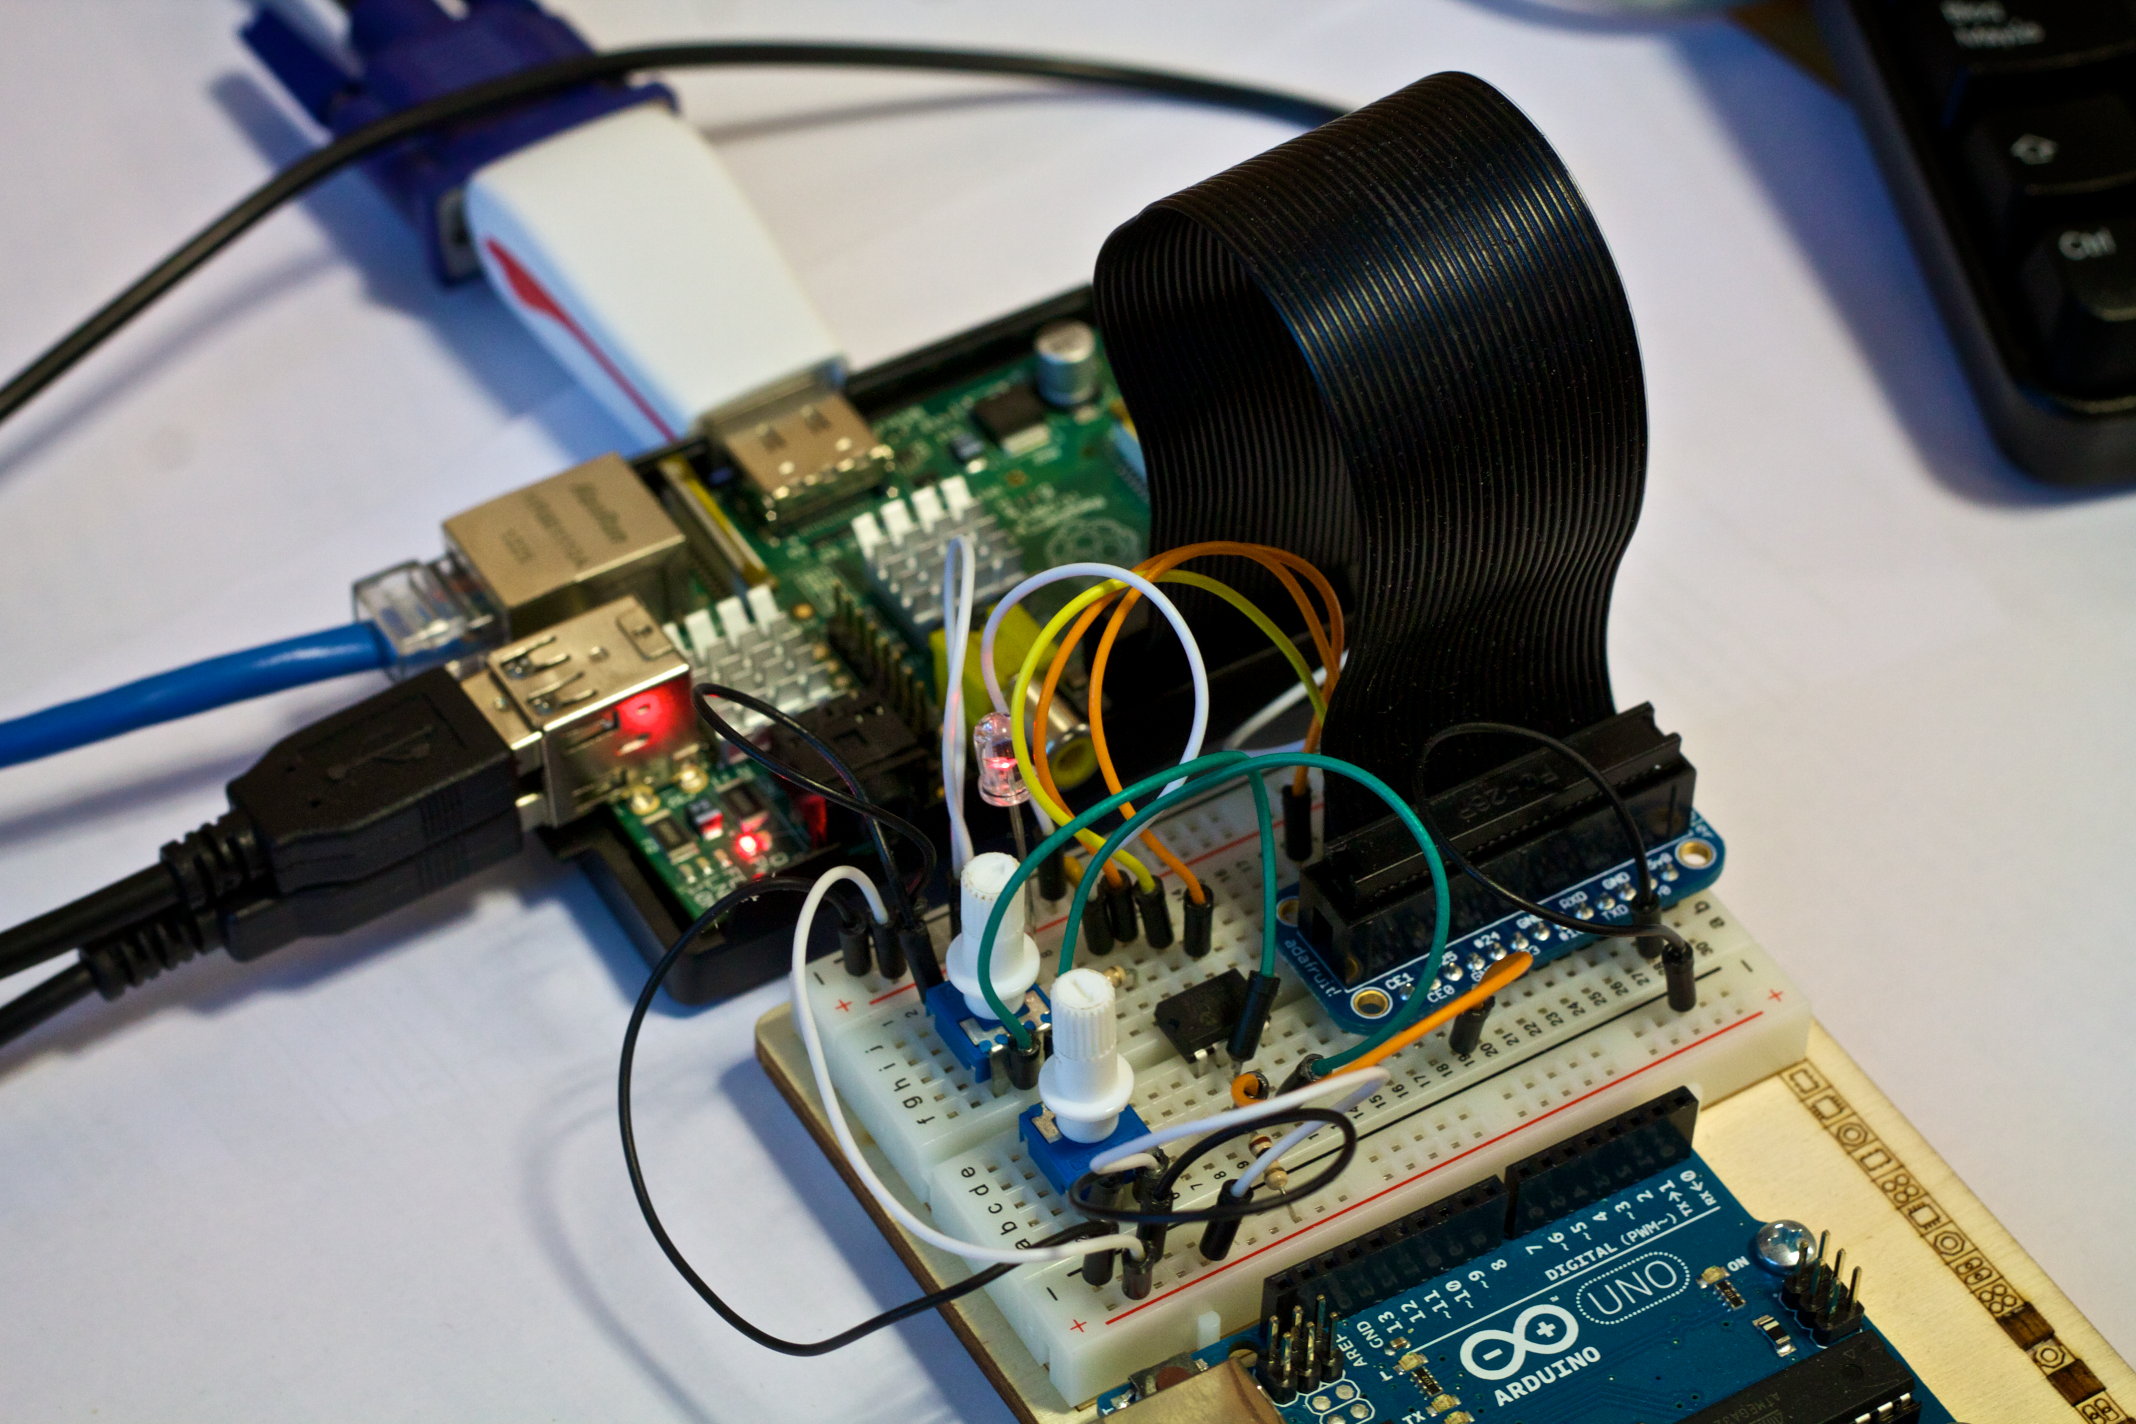
\includegraphics[width=1\textwidth]{img/proto1.png}
  			\caption{El primer prototipo conectado a la Raspberry Pi.}\label{fig:proto1}
		\end{figure}
		El primer prototipo (\autoref{fig:proto1}) cuenta con un chip convertidor analógico/digital MCP3202 que provee dos entradas analógicas y precisión de 12 bits. El chip se comunica con la Raspberry Pi a través de un interfaz de serie compatible con el protocolo SPI, la conexión con la misma es mediante los pines GPIO. Podemos controlar la tensión que lee el chip mediante dos potenciómetros conectados a sendos canales. Todo el conjunto está montado sobre una placa de prototipado o \emph{protoboard}.
		Los datos que se obtienen del mismo son voltios, concretamente entre 0 y 3,3 ya que la misma placa se alimenta de la propia Raspberry, no requiriendo así alimentación externa. Durante el desarrollo de los siguientes prototipos esto cambiará para poder conectar los sensores del interfaz original PASCO (éstos operan entre $ \pm 10 $voltios y algunos requieren alimentación extra de 5 y/o 12 voltios). 
		

	\subsection{Implementación en el programa.}
		Se ha decidido realizar la implementación de la librería directamente y prescindir de la portabilidad del programa a otros sistemas operativos dejando esta característica como una futura mejora. Al ser una librería de Python mas, con solo importarla en nuestro programa ya tenemos acceso a sus módulos, especialmente al módulo Acquisition, que es nuestro nexo de conexión.
		
		Al disponer solo de dos canales disponibles según el prototipo pero tener el interfaz gráfico preparado para cuatro canales y no tener ninguna manera de obtener a través de la librería el número de canales ofrecidos, se ha programado de manera que la interfaz gráfica intenta inicializar cada uno de los cuatro canales y si alguno falla simplemente queda marcado como ``no disponible'' y se desactivan los controles asociados al mismo en el interfaz gráfico. 
		
		\subsection{Utilización del prototipo.}
		La librería se comportó según lo acordado en el diseño, por tanto tras la integración de ésta el funcionamiento fue el esperado y los cambios en el código original fueron mínimos. En la \autoref{fig:pida_2ch_sample} se puede ver un ejemplo de su funcionamiento.
		
	\begin{figure}[H]
			\centering
		  	\includegraphics[width=1\textwidth]{img/pida_2ch_sample.png}
  			\caption{Funcionamiento del primer prototipo de dos canales.}\label{fig:pida_2ch_sample}
		\end{figure}
		\section{Segundo prototipo.}
			\begin{figure}[H]
			\centering
		  	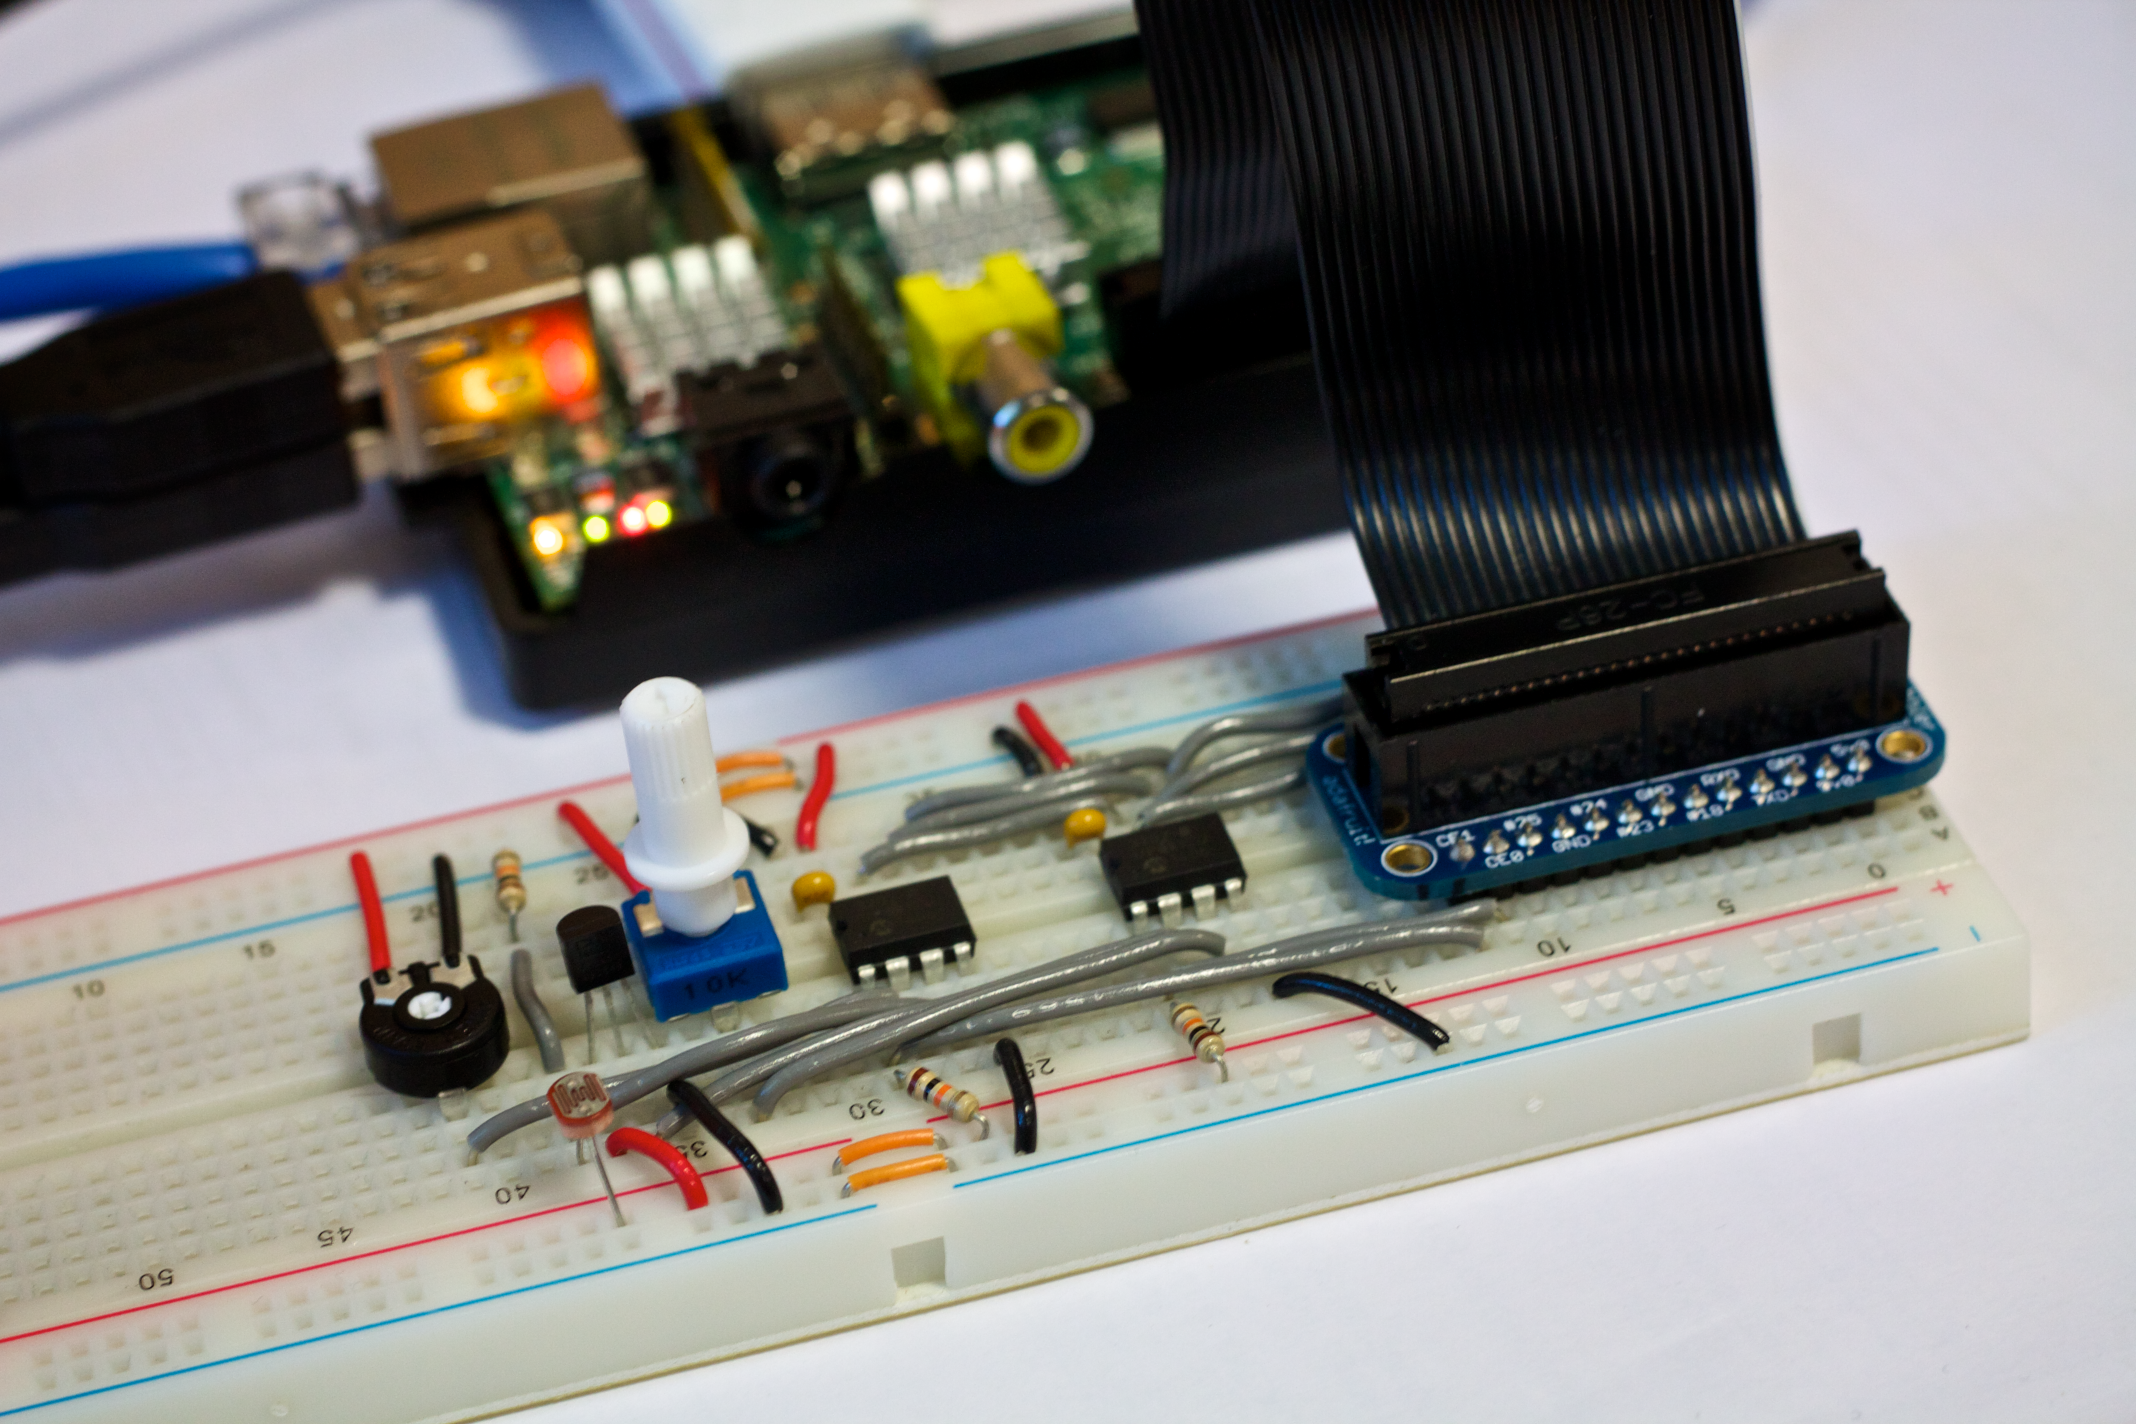
\includegraphics[width=1\textwidth]{img/proto2.png}
  			\caption{El segundo prototipo conectado a la Raspberry Pi.}\label{fig:proto2}
		\end{figure}
		El segundo prototipo (\autoref{fig:proto2}) cuenta con las mismas características que el primero pero esta vez con dos chips MCP3202 dando soporte para cuatro canales. Dos de ellos son sensores: uno de luz y otro de temperatura. La distribución de canales por tanto es la siguiente:
		\begin{itemize}
			\item Canal 0: Potenciómetro (azul).
			\item Canal 1: Sensor de temperatura
			\item Canal 2: Sensor de luz.
			\item Canal 3: Potenciómetro (negro).
		\end{itemize}

		Los sensores no se han calibrado por lo que los datos obtenidos de ellos siguen siendo voltaje entre 0 y 3,3 voltios.
		
		\subsection{Implementación y utilización en el programa.}
		El código estaba preparado para ser utilizado hasta con cuatro canales, por tanto no hizo falta acondicionar nada del mismo para la conexión del nuevo prototipo.
		
		El funcionamiento una vez más fue el esperado, recibiendo datos de los cuatro canales y toda la mecánica funcionando sin ningún problema, incluída la visualización y exportación de los datos. 
		En la \autoref{fig:pida42ch_sample} se puede ver una captura del programa funcionando a distintas frecuencias e interactuando con los distintos canales.
		
			\begin{figure}[H]
			\centering
		  	\includegraphics[width=1\textwidth]{img/pida_4ch_sample.png}
  			\caption{Funcionamiento del segundo prototipo con cuatro canales.}\label{fig:pida42ch_sample}
		\end{figure}
%\pagebreak%
\chapter{Evaluación y pruebas.}
\epigraphhead [30]{%
  \epigraph{``Las máquinas son cada vez más eficientes y mejores, por lo que queda claro que la imperfección es la grandeza del hombre."}
  {Ernst Fischer, filósofo.}%
}

En este capítulo se describen las pruebas que se han ejecutado sobre el software con el fin de ponerlo a prueba, conocer la exactitud temporal con la que los datos son medidos y sus limitaciones.

\section{Descripción de las pruebas.}
	Para la realización de este capítulo se van a obtener dos elementos: la frecuencia real a la que el sistema está tomando medidas y la carga del sistema en cada una de ellas. Para obtener el primer dato hemos calculado el intervalo medio entre medidas dividiendo el tiempo real que ha tomado la adquisición entre el número de datos y luego se ha realizado su inversa, como indica la \autoref{eq:Fr}.

\begin{equation}\label{eq:Fr}
	 		\bar{F}_{Real}=\dfrac{1}{T_{total}/n_{medidas}}
\end{equation}

	El procedimiento de las pruebas ha sido el siguiente:

\begin{itemize}
	\item Se han elaborado una serie de tests basados en la frecuencia y canales usados en la adquisición de datos para obtener una medida de cuál es la frecuencia máxima a la que se puede operar con nuestra solución actual y se ha anotado la carga del sistema para evaluar cual es el motivo de la limitación en cada caso.
	
	\item Se han adquirido datos a distintas frecuencias durante un tiempo mínimo de cinco minutos en cada caso, variando desde 1Hz hasta 2000Hz con un canal, hasta 1000Hz con dos canales simultáneamente y hasta 750Hz con cuatro canales. 
	\item Se han exportado los datos mediante el módulo interno del programa, trasladado a una hoja de cálculo y obtenido la frecuencia media real de la adquisición mediante \ref{eq:Fr}.
	\item Se ha comparado la frecuencia real obtenida en el apartado anterior con la frecuencia teórica en orden de calcular el error absoluto medio y error relativo porcentual mediante las fórmulas \ref{eq:Ea} y \ref{eq:Er} respectivamente. donde $ \bar{F_r} $ representa la frecuencia media real obtenida en \ref{eq:Fr} y F la frecuencia teórica.
	
	 	\begin{equation}\label{eq:Ea}
	 		\bar{\epsilon_{a}}=\left|\bar{F_r}-F\right|
	 	\end{equation}
		\begin{equation}\label{eq:Er}
			 \bar{\epsilon_{r}}=\left|\dfrac{\bar{F_r}-F}{F}\right|\cdot100
		\end{equation}

\end{itemize}
	Los datos se representarán en tablas con los siguientes datos:
	\begin{itemize}
		\item{F (Hz)}: Frecuencia en herzios especificada en la interfaz del programa.
		\item{T\tsub{total}}: Tiempo total de la adquisición de datos, medido en segundos.
		\item{Nº\tsub{muestras}}: Número de muestras realizadas en la adquisición.
		\item{$ ·T_{medio} $}: Intervalo medio entre medidas, especificado en segundos.
		\item{$\bar{F}_{Real}$}: Frecuencia real a la que se ha realizado la adquisición, calculado por la \autoref{eq:Fr}.
		\item{$ \bar{\epsilon_{a}} $}: Error absoluto de la frecuencia, calculado por la \autoref{eq:Ea} y medido en Hz.
		\item{$ \bar{\epsilon_{r}} $ }: Error relativo de la frecuencia, calculado por la \autoref{eq:Er}, en porcentaje (\%).
	\end{itemize}

\subsection{Carga del sistema.}
	 La carga del sistema se ha medido mediante el comando \emph{uptime}\footnote{\url{http://en.wikipedia.org/wiki/Uptime\#Linux} (en inglés)} y anotando el segundo valor de carga al representar la misma durante los últimos cinco minutos. 
	 
	 Por realizar una explicación rápida de como se mide la carga del sistema, si el valor obtenido es de 0.60, el sistema ha estado de media un 40\% del tiempo libre de carga. En cambio si es por ejemplo de 1.60, el sistema ha tenido de media un 60\% de sobrecarga, y quiere decir al ser este un sistema monoprocesador que 0.60 procesos de media han tenido que esperar para obtener tiempo de CPU\cite{wikipedia_cpuload}. Como nota, la carga del sistema en \emph{idle} (sin utilizar) es de 0.11, por tanto un 11\% del tiempo de procesamiento lo utiliza el sistema operativo.
	 
	 No se debe confundir la sobrecarga con que el sistema no es capaz de realizar la tarea especificada o que las restricciones temporales no se van a poder cumplir. Como se puede comprobar más adelante en las pruebas, el uso intensivo de la CPU por el programa no ha provocado medidas imprecisas.
	 
	 \subsection{¿Cuándo una medida no es válida y el sistema ha tocado su límite?}
	Se ha decidido que una frecuencia deja de ser precisa a partir del 0,25\% de error relativo ($ \epsilon_r$). A partir de la adquisición tachada como no válida se realiza una o dos medidas más y se comparan las cargas en el sistema en ambos casos para investigar la causa del error.
	 
	\subsection{¿De dónde puede proceder el límite?}	 
	 Los orígenes que se toman de la limitación pueden ser bien de la propia capacidad de cómputo de la Raspberry Pi, o del sistema de entrada/salida o el mismo hardware que no es capaz de entregar los datos al ritmo que se exigen. Para discernir entre ambas posibilidades hemos obtenido los siguientes niveles de carga que tiene nuestro programa sin utilizar el interfaz de adquisición mediante el uso del simulador funcionando a la máxima velocidad que nos permite el sistema:
\begin{table}[!ht]
  \centering
  \begin{tabular}{| c | c |}
  	\hline
    Número de canales activos & Carga del sistema \\ \hline
	1 			&	2.02	\\ \hline
	2 			&	2.40	\\ \hline
	4 			&	4.92	\\ \hline
  \end{tabular}
  \caption{Cargas máximas en el sistema sin utilizar el interfaz de adquisición.}
  \label{tab:test_cargas_sim}
\end{table}
	
	Por otra parte, se ha comprobado empíricamente que la carga total por la que el sistema se queda totalmente congelado e inusable es a partir de aproximadamente 5.00.
	
	Con estos valores, si la carga del sistema durante la adquisición de datos en los casos donde el error no es tolerable es similar o superior a la determinada en la \autoref{tab:test_cargas_sim}, el cuello de botella lo estará creando la Raspberry; mientras que si no es así el cuello de botella estará en el sistema de entrada/salida o el hardware de adquisición de datos, y el sistema aún tendrá recursos para ir más rápido.
	
	Destacar que la carga del sistema es un valor muy abstracto y variable, la única manera de llegar a una conclusión es mediante la realización de todas las pruebas y la puesta en común de las mismas, que se realiza al final del capítulo.
	
\section{Pruebas con un solo canal.}
	Las primeras pruebas se realizan con utilizando un solo canal adquiriendo datos a distintas frecuencias. Se recogen los resultados en la \autoref{tab:test_1ch}. 
\begin{table}[!ht]
  \centering
  \begin{tabular}{| c | c | c | c | c | c | c | }
  	\hline
    F (Hz) & T\tsub{total} (s) & Nº\tsub{muestras}& $ ·T_{medio} $ (s) & $\bar{F}_{Real}$ (Hz) & $ \bar{\epsilon_{a}} $& $ \bar{\epsilon_{r}} $ (\%) \\ \hline
	1 			&	358,0001	&	358			&	1,00000 		&	0,9999			&	3,7454E-7	&	3,7454E-5 	\\ \hline
	2 			&	324,0001	&	648			&	0,50000 		&	1,9999			&	9,0651E-7	&	4,5325E-5 	\\ \hline
	5			&	310,2001	&	1551		&	0,20000 		&	4,9999			&	2,2781E-6	&	4,5562E-5 	\\ \hline
	10		&	302,5014	&	3025		&	0,10000 		&	9,9999			&	4,8082E-5	&	0,000480 	\\ \hline
	50		&	340,2401	&	17012		&	0,02000		&	49,9999		&	1,8537E-5	&	3,7075E-5 	\\ \hline
	100		&	304,9405	&	30494		&	0,01000		&	99,9998		&	0,000168	&	0,000168 	\\ \hline
	500		&	308,0007	&	153750	&	0,00200		&	499,1871	&	0,812882	&	0,162576 	\\ \hline
	1000	&	312,9217	&	312872	&	0,001000	&	999,8411	&	0,158891	&	0,015889 	\\ \hline
	1250	&	348,1531	&	393899	&	0,000883	&	\tred{1131,392} & \tred{118,6071}	&	\tred{9,488575} 	\\ \hline
	1500	&	320,4741	&	364017	&	0,000880	&	\tred{1135,869}	&	\tred{364,1300}	&	\tred{24,27533} 	\\ \hline
	2000	&	333,6778	&	376117	&	0,000887	&	\tred{1127,186}	&	\tred{872,8139}	&	\tred{43,64069} 	\\ \hline
  \end{tabular}
  \caption{Resultados de los tests utilizando un solo canal.}
  \label{tab:test_1ch}
\end{table}
  
  
  Como se puede observar, las adquisiciones tienen un error relativo tolerable hasta los 1000Hz (por debajo del 1\%) habiendo siendo el pico más alto de un 0,16\% dado en los 500Hz y seguramente por algún fallo puntual, puesto que en la siguiente medida de 1000Hz el error es bastante inferior (0,015\%).
  
   No obstante, a partir del kilohercio hay errores del 24\% en 1500Hz y del 43\% en 2000Hz, dejando frecuencias medias de 1135,8Hz y 1127,1Hz reales respectivamente, errores ya por tanto no tolerables. 
   
   \subsection{Cargas del sistema en cada caso.}
   En la \autoref{tab:test_1chLoad} se comparan los errores con la carga del sistema.

\begin{table}[!ht]
  \centering
  \begin{tabular}{| c | c | c | c | }
  	\hline
    F (Hz) &  $ \bar{\epsilon_{a}} $& $ \bar{\epsilon_{r}} $ (\%) & Carga del sistema \\ \hline
	1 			&	3,7454E-7	&	3,7454E-5 	&	0.38 	\\ \hline
	2 			&	9,0651E-7	&	4,5325E-5 	&	0.37	\\ \hline
	5			&	2,2781E-6	&	4,5562E-5 	&	0.32	\\ \hline
	10		&	4,8082E-5	&	0,0004808 	&	0.35	\\ \hline
	50		&	1,8537E-5	&	3,7075E-5 	&	0.37	\\ \hline
	100		&	0,0001680	&	0,0001680 	&	0.52	\\ \hline
	500		&	0,8128820	&	0,1625764 	&	0.71	\\ \hline
	1000	&	0,1588911	&	0,0158891  &	1.45	\\ \hline
	1250	&	\tred{118,60719}	&	\tred{9,4885755} & 1.55	\\	 \hline
	1500	&	\tred{364,13002}	&	\tred{24,275335} & 1.68	\\ \hline
	2000	&	\tred{872,81390}	&	\tred{43,640695} & 1.69	\\ \hline
  \end{tabular}
  \caption{Comparación del error con la carga del sistema al utilizar un solo canal.}
  \label{tab:test_1chLoad}
\end{table}

Entre 1 y 100Hz la carga es prácticamente inexistente, el sistema funciona ligero y con más del 50\% de ciclos libres.

A partir de 100Hz la carga empieza a ser más notable y a crecer conforme las frecuencias suben, y a los 1000Hz el sistema lleva ya un 45\% de sobrecarga. De todos modos, la sobrecarga no es alarmante ya que el error relativo sigue siendo bajo, indicando que las restricciones temporales se cubren razonablemente.

Analizando los tres últimos valores testados donde los errores han sido muy altos, 1250Hz, 1500Hz y 2000Hz, las cargas son muy similares y por debajo de los 2.02 que consideramos en \ref{tab:test_cargas_sim} que podría correr el programa sin problema en este tipo de prueba. Por tanto se considera que el cuello de botella en este test no se encuentra en el programa por una carga excesiva en la CPU si no en la entrada/salida o el hardware de adquisición.

\section{Pruebas con dos canales simultáneamente.}
El siguiente test es con dos canales adquiriendo datos cuyos resultados se pueden ver en la \autoref{tab:test_2ch}. 
\begin{table}[!ht]
  \centering
  \begin{tabular}{| c | c | c | c | c | c | c | }
  	\hline
    F (Hz) & T\tsub{total} (s) & Nº\tsub{muestras}& $ ·T_{medio} $ (s) & $\bar{F}_{Real}$ (Hz) & $ \bar{\epsilon_{a}} $& $ \bar{\epsilon_{r}} $ (\%) \\ \hline
	\multirow{2}{*}{1} 		&	329,0002	&	328			&	1,00000 		&	0,9999			&	8,8734E-7	&	8,8734E-5 	\\
										&	329,0002	&	328			&	1,00000 		&	0,9999			&	7,2321E-7	&	7,2321E-5 	\\ \hline 
	\multirow{2}{*}{2} 		&	317,0001	&	634			&	0,50000		& 1,9999			&	8,2384E-7	&	4,1192E-5 	\\
										&	316,5001	&	633			&	0,50000		& 1,9999			&	7,6650E-7	&	3,8325E-5	\\ \hline 
										\multicolumn{7}{|c|}{. . .} \\ \hline
	%\multirow{2}{*}{5} 		&	326,6001	&	1633		&	0,20000		& 4,9999			&	2,7614E-6	&	5,5228E-5 	\\
										%&	326,0001	&	1629		&	0,20000		& 4,9999			&	2,7165E-6	&	5,4330E-5	\\ \hline 
	%\multirow{2}{*}{10}	&	363,9001	&	3630		&	0,10000		& 9,9999			&	4,4472E-6	&	4,4472E-5 	\\
										%&	363,6007	&	3636		&	0,10000		& 9,9999			&	2,1952E-5	&	0,0002195	\\ \hline 
	%\multirow{2}{*}{50}	&	391,9001	&	19595		&	0,02000		& 49,9999		&	2,3018E-5	&	4,6037E-5 	\\
										%&	391,3208	&	19566		&	0,02000		& 49,9998		&	0,0001063	&	0,0002127	\\ \hline 
	%\multirow{2}{*}{100}	&	319,1501	&	31915		&	0,01000		& 99,9999		&	4,9838E-5	&	4,9838E-5 	\\
										%&	318,6724	&	31867		&	0,01000		& 99,9992		&	0,0007617	&	0,0007617	\\ \hline 
	\multirow{2}{*}{500}	&	325,1106	&	162551	&	0,00200		& 499,9867		&	0,0132585	&	0,0026517 	\\
										&	324,6987	&	162349	&	0,00200		& 499,9987		&	0,0012213	&	0,0002442	\\ \hline 
	\multirow{2}{*}{750}	&	319,3583	&	199363	&	0,00160		& \tred{624,2611}	&	\tred{125,7388}	&	\tred{16,76517} 	\\
										&	318,8745	&	201618	&	0,00158		& \tred{632,2799}	&	\tred{117,7200}	&	\tred{15,69601}	\\ \hline 
	\multirow{2}{*}{1000}&	349,3195	&	219508	&	0,00159		& \tred{628,3873}	&	\tred{371,6126}	&	\tred{37,16126} 	\\
										&	348,9656	&	216182	&	0,00161		& \tred{619,4936}	&	\tred{380,5063}	&	\tred{38,05063}	\\ \hline 
  \end{tabular}
  \caption{Resultados de los tests utilizando dos canales.}
  \label{tab:test_2ch}
\end{table}

	En este caso el error relativo se dispara a partir de los 500Hz, teniendo en los tests a 750Hz una frecuencia real de algo más de 624Hz y 632Hz en cada canal, sugiriendo que el límite para este tipo de adquisición se encuentra alrededor de esos valores.. En los casos precedentes el error sigue siendo contenido y satisfactorio dada la naturaleza de propósito general de este sistema. Se han ignorado los valores entre 2Hz y 500Hz al ser todos muy parecidos y no aportar nada al lector.

   \subsection{Cargas del sistema en cada caso.}
	En la \autoref{tab:test_2chLoad} se comparan los resultados con las cargas del sistema.
	 
\begin{table}[!ht]
  \centering
  \begin{tabular}{| c | c | c | c | }
  	\hline
    F (Hz) &  $ \bar{\epsilon_{a}} $& $ \bar{\epsilon_{r}} $ (\%) & Carga del sistema \\ \hline
	\multirow{2}{*}{1} 		&	8,8734E-7	&	8,8734E-5 	& \multirow{2}{*}{0.24}\\
										&	7,2321E-7	&	7,2321E-5 	&	\\ \hline 
	\multirow{2}{*}{2} 		&	8,2384E-7	&	4,1192E-5 	& \multirow{2}{*}{0.32}\\
										&	7,6650E-7	&	3,8325E-5	&	\\ \hline 
	\multirow{2}{*}{5} 		&	2,7614E-6	&	5,5228E-5 	& \multirow{2}{*}{0.32}\\
										&	2,7165E-6	&	5,4330E-5	&	\\ \hline 
	\multirow{2}{*}{10}	&	4,4472E-6	&	4,4472E-5 	& \multirow{2}{*}{0.33}\\
										&	2,1952E-5	&	0,0002195	&	\\ \hline 
	\multirow{2}{*}{50}	&	2,3018E-5	&	4,6037E-5 	& \multirow{2}{*}{0.43}\\
										&	0,0001063	&	0,00021274&	\\ \hline 
	\multirow{2}{*}{100}	&	4,9838E-5	&	4,98389E-5 	& \multirow{2}{*}{0.56}\\
										&	0,0007617	&	0,00076173	&	\\ \hline 
	\multirow{2}{*}{500}	&	0,0132585	&	0,00265171 	& \multirow{2}{*}{1.36}\\
										&	0,0012213	&	0,00024427	&	\\ \hline 
	\multirow{2}{*}{750}	&	\tred{125,7388}	&	\tred{16,76517} & \multirow{2}{*}{1.80}\\
										&	\tred{117,7200}	&	\tred{15,69601}	&	\\ \hline 
	\multirow{2}{*}{1000}&	\tred{371,6126}	&	\tred{37,16126}	& \multirow{2}{*}{2.08}\\
										&	\tred{380,5063}	&	\tred{38,05063}	&	\\ \hline 
  \end{tabular}
  \caption{Comparación del error con la carga del sistema al utilizar dos canales.}
  \label{tab:test_2chLoad}
\end{table}

	El sistema comienza a sobrecargarse en los 500Hz pero al igual que en las pruebas anteriores, este 36\% extra de procesamiento no compromete la frecuencia a la que se toman los datos ya que los errores siguen siendo muy bajos.
	
	No obstante, los dos valores donde el error se dispara, 750Hz y 1000Hz, la sobrecarga alcanza en este último caso el 108\%  frente a los 140\% estimados en  \ref{tab:test_cargas_sim} y puede indicar que en este caso la capacidad de la propia Raspberry Pi es la limitante. Pero volviendo a los datos sobre la frecuencia media real de estos dos casos en la \autoref{tab:test_2ch} se puede observar que la suma de la misma en cada caso son 1256,541Hz y 1247,880Hz, cuando el caso límite de las pruebas con un solo canal arrojaron una frecuencia límite de 1135,8Hz. Los valores son muy próximos entre sí por lo que realmente no queda claro si puede ser una cosa u otra.



\section{Pruebas con cuatro canales simultáneamente.}
Las últimas pruebas corresponden a las realizadas con cuatro canales adquiriendo datos simultáneamente y cuyos resultados se pueden ver en la \autoref{tab:test_4ch}.

	Se han vuelto a ignorar los resultados entre 2Hz y 250Hz al no ser útiles para el lector. En este caso el funcionamiento es aceptable hasta el test de los 500Hz, donde el error supera el 35\% en todos los canales y la frecuencia media real es de casi 317Hz en el canal más lento. 
	
	Se puede comprobar como parece haber un límite global en la frecuencia en la que el interfaz puede funcionar ya que la suma de todas las frecuencias medias reales obtenidas en 500Hz es 1284,06Hz y a 750Hz es 1286,831Hz, tal y como se sugirió en la prueba anterior obteniendo un límite máximo de 1256,541Hz y en la primera prueba con 1135,8Hz.
	
	
	
		\begin{table}[H]
  \centering
  \begin{tabular}{| c | c | c | c | c | c | c | }
  	\hline
    F (Hz) & T\tsub{total} (s) & Nº\tsub{muestras}& $ ·T_{medio} $ (s) & $\bar{F}_{Real}$ (Hz) & $ \bar{\epsilon_{a}} $& $ \bar{\epsilon_{r}} $ (\%) \\ \hline
	\multirow{4}{*}{1} 		&	322,0001	&	323			&	1,00000 		&	0,9999			&	5,6303E-7	&	5,6303E-5	\\
										&	322,0001	&	323			&	1,00000 		&	0,9999			&	4,5744E-7	&	4,5744E-5 	\\
										&	322,0001	&	323			&	1,00000 		&	0,9999			&	4,8540E-7	&	4,8540E-5 	\\
										&	322,0001	&	323			&	1,00000 		&	0,9999			&	4,6055E-7	&	4,6055E-5 	\\ \hline 
	\multirow{4}{*}{2} 		&	322,5001	&	646			&	0,50000 		&	1,9999			&	1,0587E-6	&	5,2939E-5	\\
										&	322,5001	&	646			&	0,50000 		&	1,9999			&	1,2282E-6	&	6,1413E-5	\\
										&	322,5001	&	646			&	0,50000 		&	1,9999			&	1,0735E-6	&	0,0000536 	\\
										&	322,5001	&	646			&	0,50000 		&	1,9999			&	9,4368E-7	&	4,7184E-5 	\\ \hline 
	%\multirow{4}{*}{5} 		&	380,4001	&	1903		&	0,20000 		&	4,9999			&	1,7358E-6	&	3,4716E-5	\\
	%									&	380,4007	&	1903		&	0,20000 		&	4,9999			&	9,3425E-6	&	0,0001868	\\
	%									&	380,4003	&	1903		&	0,20000 		&	4,9999			&	4,5575E-6	&	9,1151E-5 	\\
	%									&	380,4002	&	1903		&	0,20000 		&	4,9999			&	3,0716E-6	&	6,1433E-5 	\\ \hline 
	%\multirow{4}{*}{10}	&	358,0001	&	3581		&	0,10000 		&	9,9999			&	4,8712E-6	&	4,8712E-5	\\
	%									&	357,9001	&	3580		&	0,10000 		&	9,9999			&	4,2986E-6	&	4,2986E-5	\\
	%									&	358,0004	&	3581		&	0,10000 		&	9,9999			&	1,1686E-5	&	0,0001168 	\\
	%									&	358,0007	&	3581		&	0,10000 		&	9,9999			&	2,2300E-5	&	0,0002230 	\\ \hline
	%\multirow{4}{*}{50}	&	383,6407	&	19183		&	0,02000 		&	49,9999		&	9,3884E-5	&	0,0001877	\\
	%									&	383,6201	&	19182		&	0,20000 		&	49,9999		&	0,0000194	&	3,8860E-5	\\
	%									&	383,6401	&	19183		&	0,20000 		&	49,9999		&	1,9863E-5	&	3,9726E-5 	\\
	%									&	383,7539	&	19188		&	0,20000 		&	49,9981		&	0,0018233	&	0,0036467 	\\ \hline
	%\multirow{4}{*}{100}	&	312,7971	&	31280		&	0,01000 		&	99,9977		&	0,0022902	&	0,0022902	\\
	%									&	312,8002	&	31281		&	0,01000 		&	99,9999		&	6,6360249	&	6,6360E-5	\\
	%									&	312,8826	&	31287		&	0,01000 		&	99,9927		&	0,0072389	&	0,0072389 	\\
	%									&	312,9006	&	31291		&	0,01000 		&	99,9997		&	0,0002015	&	0,0002015 	\\ \hline
%
\multicolumn{7}{|c|}{. . .} \\ \hline
	\multirow{4}{*}{250}	&	327,0160	&	81738		&	0,00400 		&	249,9479	&	0,0520258	&	0,0208103	\\
										&	327,0132	&	81739		&	0,00400 		&	249,9532	&	0,0467881	&	0,0187152	\\
										&	327,0402	&	81761		&	0,00400 		&	249,9997	&	0,0002219	&	8,8778E-5 	\\
										&	327,0321	&	81759		&	0,00400 		&	249,9998	&	0,0001128	&	4,5144E-5 	\\ \hline
	\multirow{4}{*}{500}	&	347,3804	&	112507	&	0,00308 		&	\tred{323,8696}	&	\tred{176,13030}	&	\tred{35,22606}	\\
										&	347,3536	&	111828	&	0,00310 		&	\tred{321,9398}	&	\tred{178,06011}	&	\tred{35,61202}	\\
										&	347,3543	&	111592	&	0,00311 		&	\tred{321,2598}	&	\tred{178,74013}	&	\tred{35,74802}	\\
										&	347,8928	&	110281	&	0,00315 		&	\tred{316,9941}	&	\tred{183,00588}	&	\tred{36,60117}	\\ \hline
	\multirow{4}{*}{750}	&	335,8788	&	107725	&	0,00311 		&	\tred{320,7228}	&	\tred{429,27716}	&	\tred{57,23695}	\\
										&	335,9379	&	107917	&	0,00311 		&	\tred{321,2379}	&	\tred{428,76208}	&	\tred{57,16827}	\\
										&	335,9450	&	108357	&	0,00310 		&	\tred{322,5408}	&	\tred{427,45914}	&	\tred{56,99455}	\\
										&	335,9791	&	108291	&	0,00310 		&	\tred{322,3116}	&	\tred{427,68835}	&	\tred{57,02511}	\\ \hline
  \end{tabular}
    \caption{Resultados de los tests utilizando los cuatro canales.}\label{tab:test_4ch}
\end{table}
	
	   \subsection{Cargas del sistema en cada caso.}
	En la \autoref{tab:test_4chLoad} se puede ver la comparación de los errores con la carga del sistema (C\tsub{S}) en cada caso.

  \label{tab:text_4chLoad}
	Con cuatro canales no parece ser diferente al resto de pruebas con menos canales y aunque en los casos donde el error es alto la carga en el sistema también es importante, no llega al nivel máximo especificado en la \autoref{tab:test_cargas_sim} (esta vez 2.36 frente a 4.92), y en ambos casos es similar entre sí (2.33 y 2.36). 
	
	Una vez más, no es la capacidad de cálculo la que nos está limitando la frecuencia de los canales. Esta vez se ve más claramente ya que si se hace el recuento de hilos que se están ejecutando (un hilo por cada canal de adquisición, otro hilo de actualización de la gráfica y el hilo principal) no puede ser que el sistema esté sobrecargado cuando solo 1.36 procesos tienen que esperar tiempo de CPU y hay al menos seis ejecutándose en nuestro programa.

%		\pagebreak
		
\begin{table}[H]
  \centering
  \begin{tabular}{| c | c | c | c | c | c | c | c | c | }
  	\cline{1-4}\cline{6-9}
    F (Hz) &  $ \bar{\epsilon_{a}} $& $ \bar{\epsilon_{r}} $ (\%) & C\tsub{S} & \multirow{9}{*}{} & F (Hz) &  $ \bar{\epsilon_{a}} $& $ \bar{\epsilon_{r}} $ (\%) & C\tsub{S}\\   	\cline{1-4}\cline{6-9}
    \multirow{4}{*}{1} 		&	5,6303E-7	&	5,6303E-5	&	\multirow{4}{*}{0.26}  & & \multirow{4}{*}{100}	&	0,0022902	&	0,0022902	&	\multirow{4}{*}{1.64}	\\
										&	4,5744E-7	&	4,5744E-5 	&	&	& &	6,6360249	&	6,6360E-5	&	\\
										&	4,8540E-7	&	4,8540E-5 	&	&	& &	0,0072389	&	0,0072389 	&	\\
										&	4,6055E-7	&	4,6055E-5 	&	&	& &	0,0002015	&	0,0002015 	&	\\ \cline{1-4}\cline{6-9}
	\multirow{4}{*}{2} 		&	1,0587E-6	&	5,2939E-5	&	\multirow{4}{*}{0.35} &	& 	\multirow{4}{*}{250}	&	0,0520258	&	0,0208103	&	\multirow{4}{*}{2.12}	\\
										&	1,2282E-6	&	6,1413E-5	& & & &	0,0467881	&	0,0187152	&	\\
										&	1,0735E-6	&	0,0000536 	&	& & &	0,0002219	&	8,8778E-5 	&	\\
										&	9,4368E-7	&	4,7184E-5 	& & & &	0,0001128	&	4,5144E-5 	&	\\ \cline{1-4}\cline{6-9}
	\multirow{4}{*}{5} 		&	1,7358E-6	&	3,4716E-5	&	\multirow{4}{*}{0.38} & & \multirow{4}{*}{500}	&	\tred{176,13030}	&	\tred{35,22606}		&	\multirow{4}{*}{2.33}\\
										&	9,3425E-6	&	0,0001868	& & & &	\tred{178,06011}	&	\tred{35,61202}		&	\\
										&	4,5575E-6	&	9,1151E-5 	&	& & &	\tred{178,74013}	&	\tred{35,74802}		&	\\
										&	3,0716E-6	&	6,1433E-5 	&	& & &	\tred{183,00588}	&	\tred{36,60117}		&	\\ \cline{1-4}\cline{6-9}
	\multirow{4}{*}{10}	&	4,8712E-6	&	4,8712E-5	&	\multirow{4}{*}{0.56} & & \multirow{4}{*}{750}	&	\tred{429,27716}	&	\tred{57,23695}		&	\multirow{4}{*}{2.36}\\
										&	4,2986E-6	&	4,2986E-5	&	& & &	\tred{428,76208}	&	\tred{57,16827}		&	\\
										&	1,1686E-5	&	0,0001168 	&	& & &	\tred{427,45914}	&	\tred{56,99455}		&	\\
										&	2,2300E-5	&	0,0002230 	&	& & &	\tred{427,68835}	&	\tred{57,02511}		&	\\  \cline{1-4}\cline{6-9}
	\multirow{4}{*}{50}	&	9,3884E-5	&	0,0001877	&	\multirow{4}{*}{0.63}\\
										&	0,0000194	&	3,8860E-5	&	\\
										&	1,9863E-5	&	3,9726E-5 	&	\\
										&	0,0018233	&	0,0036467 	&	\\ \cline{1-4}
  \end{tabular}
  \caption{Comparación del error con la carga del sistema al utilizar los cuatro canales.}
  \label{tab:test_4chLoad}
\end{table}	
	

\section{Puesta en común de los resultados y conclusión.}
	\subsection{El límite.}
		En las pruebas se ha detectado un patrón de limitación por el que el interfaz tiene una frecuencia máxima total a la que puede funcionar en todo caso independientemente del número de canales.\\
\begin{wraptable}{l}{0.28\textwidth}
  \begin{tabular}{| c | c |}
  	\hline
  	Canales & $ \sum F_{max} $ 	\\ \hline
  	1			&	1135.869				\\
  	2			&	1256.541				\\
  	4			&	1286.831				\\	 \hline
  \end{tabular}
  \caption[Frecuencias máximas obtenidas por cada canal.]{F\tsub{max} por canal.}
  \label{tab:test_FMax}
\end{wraptable}
Como se puede ver en la \autoref{tab:test_FMax}, el interfaz alcanza un umbral cercano a los 1300Hz  del que no es capaz de pasar. 

Se puede asegurar por tanto aplicando una margen de error del 10\% en el peor de los valores máximos obtenidos que esta solución funciona en unos umbrales de precisión seguros siempre y cuando la suma de las frecuencias de todos los canales no supere los 1000Hz aproximadamente.
\linebreak
	\subsection{El porqué del límite.}
Descartada la limitación de la CPU (conclusión del test de cuatro canales en \ref{tab:text_4chLoad}) y comprobado que el sistema admite más carga de la que se está obteniendo en las pruebas con el interfaz (ver \autoref{tab:test_cargas_sim}) se achacan la falta de rendimiento al sistema de entrada/salida que parece no proveer de los datos a la velocidad necesaria a partir de dichas frecuencias y por tanto hace al software esperar ocioso.

Por tanto, se debe proceder al cambio de interfaz E/S o la optimización del mismo si se desean realizar medidas a frecuencias por encima de las obtenidas en estas pruebas.
%\pagebreak
\chapter{Conclusiones y trabajos futuros.}
\epigraphhead [30]{%
  \epigraph{``Ningún conocimiento humano puede ir más allá de su experiencia.''}%
  {John Locke, filósofo.}%
}

\section{Conclusiones personales.}
	Desde el principio he querido realizar un proyecto relacionado de alguna manera con una Raspberry Pi o un SBC con el objetivo de demostrar que muchas de las soluciones informáticas que hay en el mundo real en distintos ámbitos, especialmente en sistemas embebidos, son excesivas y pueden realizarse con presupuestos muy inferiores. Esto en parte es posible gracias al \emph{Open Source} tanto referido al software como al hardware y la Raspberry Pi es totalmente libre en los dos ámbitos.
	
	Este proyecto ha demostrado que efectivamente es posible abaratar costes y realizar soluciones viables mediante el uso de estos ordenadores de bajo coste, además de suponerme un desafío en general. No solo porque es el proyecto de fin de carrera donde uno ha de poner en práctica todos los conocimientos adquiridos durante estos años, sino porque además he tenido que convivir con otro proyecto paralelo con el que se perseguía un objetivo común. 
	
	Ésto ha provocado un montón de acondicionamiento e incertidumbre durante todo el proceso. Pero como en todo trabajo en equipo, la buena comunicación y la ayuda mutua han cumplido su cometido y hemos podido cumplir no todos, pero gran parte de los objetivos cuando en las primeras reuniones no se tenía claro si realmente esta solución iba a ser viable.
	
	Es otra de las razones que han hecho de este proyecto un desafío: No se sabía exactamente si la plataforma iba a ser capaz de sustituir a un equipo mucho más caro, lo cual lo ha provocado que una buena parte del mismo haya sido un estudio de viabilidad e investigación. 
	
	Personalmente estoy contento con el resultado. Si bien es un trabajo que puede llegar mucho más lejos, se ha demostrado lo que quería probar en primer lugar, y en el proceso he podido aprender un método de trabajo nuevo, un lenguaje de programación importante como Python, y además en la realización de esta memoria también he conocido \LaTeX  y gran parte de su potencia.
	
	
\section{Conclusiones profesionales.}
	El trabajo colaborativo ha sido sin duda el pilar más importante de este proyecto, puesto que de otra manera no habría sido posible llegar a donde se ha llegado. Ambos proyectandos provenimos de distintas carreras, yo por una parte de Ingeniería Informática y mi compañero de Ingeniería de Telecomunicaciones. Cada uno se ha centrado en su campo de estudio y ha sacado su parte adelante respetando la opuesta para que al final la unión de ambas haya sido un éxito.
	
	
\section{Trabajos futuros.}
	\subsection{Nuevas funcionalidades..}
		Además de las funcionalidades que no se han desarrollado por no ser un objetivo del proyecto pero se han propuesto y en ocasiones preparado a falta de escribir el modelo como la exportación PDF o la utilización del mismo en otros sistemas operativos, este programa puede albergar otras funcionalidades como por ejempo la obtención de estadísticos con los datos obtenidos.
		
	\subsection{Optimización de la solución.}
		Aunque el rendimiento actual es aceptable y muy válido, siempre se puede optimizar por ejemplo utilizando una versión del sistema operativo para tiempo real o modificando éste para que la integración en el mismo sea total, recortando programas y servicios que no resulten útiles para el propósito de este programa.
		
		También es posible conseguir una mejora a través de un estudio de la optimización del diseño de la aplicación o portando la solución a lenguajes más eficientes como puede ser C.
		
	\subsection{Adaptación a otras SBCs.}
	La Raspberry Pi es realmente la SBC menos potente de todas, sería interesante hacer el programa compatible con su clon de doble núcleo la Banana Pi. 
	
	Se dispuso de una unidad durante el desarrollo y se comprobó que el funcionamiento el programa y todo el sistema en general era muchísimo más ligero. Solo se pudo probar el funcionamiento con el simulador de datos ya que la librería piDA no está adaptada a trabajar con una Banana Pi, pero una vez realizada esa adaptación sería interesante ver de qué es capaz esta placa con toda su potencia y tan solo 20€ más de sobreprecio con respecto a la Raspberry Pi. Es muy probable que resulte en una solución más viable.
	
	\subsection{Integración del producto final en los laboratorios de la Facultad.}
	La solución funcional podría integrarse a pequeña escala en los laboratorios de la Facultad con el fin de que los alumnos hagan uso de ella. Se puede evaluar así la utilidad de la misma y la calidad en el propio entorno para el que ha sido diseñada, obteniendo así comentarios y opiniones del usuario final muy útiles.
	
	\subsection{Explotación comercial.}
	Sí la integración en los laboratorios de la Facultad es un éxito, se puede dar el paso a crear un producto comercial. La explotación del mismo empezaría por una producción industrial de la interfaz de adquisición de datos y su venta vía web. 
	
	Si realmente es un producto funcional y supone un ahorro tan grande con respecto a las soluciones de la competencia puede resultar una fuente de ingresos que remunere el esfuerzo y la idea que ha habido tras el mismo.
%\pagebreak

%\include{cap9}
%\pagebreak

% Apéndices
\appendix
%\include{apen1}
\pagebreak
%\include{apen2}
\pagebreak
%\include{apen3}
\pagebreak


% Definimos el encabezado y pie de página
\fancyhead{}
\fancyhead[LE,RO]{\thepage}
\fancyhead[LO,ER]{\rightmark}

% Glosario de términos
%\printglossary


% Bibliografía
%\bibliographystyle{empty}
%\bibliography{biblio}

%\chapter{Bibliografía.}
%\epigraphhead [30]{%
%  \epigraph{``Ni el más sabio conoce el fin de todos los caminos.''}%
%  {John Ronald Reuel Tolkien, escritor.}%
%}

\begin{thebibliography}{99}

\bibitem{VerifiedPeripherals_vga}
  eLinux.org,
  \emph{Raspberry Pi Verified Peripherals}. VGA Cables and converter boxes.  [Fecha de consulta: 15 Febrero 2014] \\
  \url{http://elinux.org/RPi_VerifiedPeripherals#HDMI-.3EVGA_Cables}

\bibitem{amazon_SD4GB}
	Amazon.es,
	\emph{Departamento de informática.}
	 Tarjeta de memoria SDHC 4GB. [Fecha de consulta: 22 Agosto 2014] \\
	\url{http://www.amazon.es/Transcend-TS4GSDHC10-Tarjeta-memoria-SecureDigital/dp/B002WE6CTU/}
	  
\bibitem{dhgate_vga}
	DHgate.com,
	\emph{China Wholesale.}
	HDMI to VGA Output Projector Monitors Adapter. [Fecha de consulta: 18 Febrero 2014] \\
	\url{http://www.dhgate.com/product/hdmi-to-vga-output-projector-monitors-adapter/170509392.html}
	
\bibitem{amazon_tecladousb}
	Amazon.es,
	\emph{Departamento de informática.}
	Genius - Teclado Kb-110X Black Usb. [Fecha de consulta: 22 Agosto 2014] \\
	\url{http://www.amazon.es/Genius-Teclado-Kb-110X-Black-Usb/dp/B005E08ADU/}
	
\bibitem{amazon_ratonusb}
	Amazon.es,
	\emph{Departamento de informática.}
	Genius XScroll - Ratón óptico con cable USB. [Fecha de consulta: 22 Agosto 2014] \\
	\url{http://www.amazon.es/Genius-XScroll-Raton-Optico-cable/dp/B000EHPPZ4/}
	
\bibitem{amazon_cargadorusb}
	Amazon.es,
	\emph{Departamento de electrónica.}
	Samsung - Cargador de móvil. [Fecha de consulta: 22 Agosto 2014] \\
	\url{http://www.amazon.es/Samsung-ETA0U10EBECSTD-Cargador-movil-red/dp/B004S6NUNG/}

\bibitem{wikipython_ide}
	Python.org,
	\emph{The Python Wiki.}
	Integrated Development Environments. [Fecha de consulta: 5 Marzo 2014] \\
	\url{https://wiki.python.org/moin/IntegratedDevelopmentEnvironments}
		
\bibitem{wikipython_guiprogramming}
	Python.org,
	\emph{The Python Wiki.}
	GUI Programming in Python. [Fecha de consulta: 5 Marzo 2014] \\
	\url{https://wiki.python.org/moin/GuiProgramming}
	
\bibitem{effbot_introductiontkinter}
	Effbot.org,
	\emph{Tkinterbook.}
	An Introduction To Tkinter. [Fecha de consulta: 5 Marzo 2014] \\
	\url{http://effbot.org/tkinterbook/tkinter-index.htm}

\bibitem{wxwidgets}
	WxWidgets,
	\emph{A Cross-Platform GUI Library.} [Fecha de consulta: 1 Abril 2014] \\
	\url{http://www.wxwidgets.org/}

\bibitem{wxpython_apifea}
	WxPython.org,
	\emph{API Documentation.}
	WX Package. [Fecha de consulta: 1 Abril 2014] \\
	\url{http://www.wxpython.org/docs/api/wx-module.html}
	
\bibitem{wxpython_apiphoenix}
	WxPython.org,
	\emph{Phoenix API Documentation.}
	Core Classes. [Fecha de consulta: 9 Abril 2014] \\
	\url{http://wxpython.org/Phoenix/docs/html/1classindex.html}
	
\bibitem{wikipython_plotting}
	Python.org,
	\emph{The Python Wiki.}
	Graphical Representations of Data. [Fecha de consulta: 20 Marzo 2014] \\
	\url{https://wiki.python.org/moin/NumericAndScientific/Plotting}
	
\bibitem{matplotlib_home}
	Matplotlib.org,
	\emph{Python 2D plotting library.} [Fecha de consulta: 20 Marzo 2014] \\
	\url{http://matplotlib.org/}
	
\bibitem{adobe_fireworks}
	Adobe.com,
	\emph{Adobe Creative Cloud.} Adobe Fireworks. [Fecha de consulta: 22 Julio 2014] \\
	\url{https://creative.adobe.com/products/fireworks}
	
\bibitem{wikipedia_cpuload}
	Wikipedia.org,
	\emph{Load (computing).} Unix-style load calculation. [Fecha de consulta: 15 Agosto 2014] \\
	\url{http://en.wikipedia.org/wiki/Load_(computing)#Unix-style_load_calculation}
	
\bibitem{errores}
	Facultad de Ciencias Exactas y Naturales de la Universidad de Antioquia,
	\emph{Laboratorio de Física}, Cuantificación de errores. [Fecha de consulta: 15 Agosto 2014] \\
	\url{http://fisica.udea.edu.co/~lab-gicm/Labratorio_Fisica_1_2012/2012_Cuantificacion\%20de\%20errores.pdf}
\end{thebibliography}









\end{document}
